\documentclass[12pt]{article}

\usepackage{amsmath, color}
\usepackage{mdwmath}
\usepackage{amssymb, epsf, epsfig, textcomp}
\renewcommand{\baselinestretch}{1.3}
\usepackage{a4wide}
\newcommand{\argmin}{\mathop{\mathrm{argmin}}}
\usepackage{caption}
\usepackage{subcaption}
\usepackage{mathtools}
\usepackage{listings}
\lstdefinestyle{myCustomMatlabStyle}{
basicstyle=\ttfamily\tiny,
breaklines=true,
language=Matlab,
numbers=left,
stepnumber=1,
numbersep=10pt,
tabsize=4,
showspaces=false,
showstringspaces=false
}

\usepackage{sectsty}

\sectionfont{\fontsize{12}{15}\selectfont}

\begin{document}
	\noindent\rule{\textwidth}{2pt}
	\begin{center}
		{\bf Technical University of Crete}\\
		{\bf School of Electrical and Computer Engineering} \\
		Course: {\bf Convex Optimization} \\
		Exercise 2 (110/500) \\
		Report Delivery Date: 17 November 2021 \\
		Instructor: Athanasios P. Liavas \\
	\end{center}
	{\bf Student: }Alevrakis Dimitrios 2017030001\\
	\rule{\textwidth}{.5pt}
	\vskip .1cm
	\noindent
	
	\begin{enumerate}
	\item[{\bf A.}]We consider a simple quadratic optimization problem.
		Let $f:\mathbb{R}^n \rightarrow \mathbb{R}$. For fixed ${\bf x}\in\mathbb{R}$ and $m>0$, let $g_{\bf x}:\mathbb{R}^n \rightarrow\mathbb{R}$ be defined as\\
		\begin{equation}
			g_{\bf x}({\bf y})\coloneqq f({\bf x})+\nabla f({\bf x})^T({\bf y}-{\bf x})+\frac{m}{2}||{\bf y}-{\bf x}||_2^2
		\end{equation}
		\begin{enumerate}
		\item[i.] We will be calculating $\nabla g_{\bf x}({\bf y})$:\\
		First we will bring $g_{\bf x}({\bf y})$ in the form:\\
		$g_{\bf x}({\bf y})=\frac{1}{2}{\bf y}^TP{\bf y}+q^T{\bf y}+r$, where $P\in \mathbb{R}^{nxn},\ P=P^T,\ q\in \mathbb{R}^n$ and $r\in\mathbb{R}$
		\begin{equation}
			\begin{split}
				g_{\bf x}({\bf y})&=f({\bf x})+\nabla f({\bf x})^T({\bf y}-{\bf x})+\frac{m}{2}||{\bf y}-{\bf x}||_2^2\\
				&=f({\bf x})+\nabla f({\bf x})^T{\bf y}-\nabla f({\bf x})^T{\bf x}+\frac{m}{2}({\bf y}-{\bf x})^T({\bf y}-{\bf x})\\
				&=f({\bf x})-\nabla f({\bf x})^T{\bf x}+\nabla f({\bf x})^T{\bf y}+\frac{m}{2}({\bf y}^T-{\bf x}^T)({\bf y}-{\bf x})\\
				&=f({\bf x})-\nabla f({\bf x})^T{\bf x}+\nabla f({\bf x})^T{\bf y}+\frac{m}{2}({\bf y}^T{\bf y}-{\bf y}^T{\bf x}-{\bf x}^T{\bf y}+{\bf x}^T{\bf x})\\
				&\overset{{\bf y}^T{\bf x}={\bf x^T}{\bf y}}{=}f({\bf x})-\nabla f({\bf x})^T{\bf x}+\nabla f({\bf x})^T{\bf y}+\frac{m}{2}({\bf y}^T{\bf y}-2{\bf x}^T{\bf y}+{\bf x}^T{\bf x})\\
				&=f({\bf x})-\nabla f({\bf x})^T{\bf x}+\frac{m}{2}{\bf x}^T{\bf x}+(\nabla f({\bf x})-m{\bf x})^T{\bf y}+\frac{1}{2}{\bf y}^Tm\mathbb{I}_n{\bf y}
			\end{split}
		\end{equation}
		Where $\mathbb{I}_n\in \mathbb{R}_{nxn}$ the identity matrix. For $\mathbb{I}_n$ is also true that $\mathbb{I}_n=\mathbb{I}^T_n$\\
		Therefore we have:
		\begin{equation}
			\begin{split}
				P&=m\mathbb{I}_n\\
				q&=\nabla f({\bf x})-m{\bf x}\\
				r&= f({\bf x})-\nabla f({\bf x})^T{\bf x}+\frac{m}{2}{\bf x}^T{\bf x}
			\end{split}
		\end{equation}
		and $\nabla g_{\bf x}({\bf y})=P{\bf y}+q =m\mathbb{I}_n y+\nabla f({\bf x})-m{\bf x} =my+\nabla f({\bf x})-m{\bf x}$
		
		\item [ii.] In order to find the optimal point and value we will prove that $g_{\bf x}{\bf y}$ is strictly convex and then set $\nabla g_{\bf x}{\bf y} = 0$.
		\begin{itemize}
			\item 
			Since $g_{\bf x}({\bf y})$ is quadratic, it is sufficient to prove that $P$ is definite positive.\\
			By definition a matrix $M \in \mathbb{R}^{nxn}$ is definite positive if ${\bf z}^TM{\bf z}>0\forall z\in\mathbb{R}^n-{0}$.
			\begin{equation}
				{\bf z}^TP{\bf z}={\bf z}^Tm\mathbb{I}_n {\bf z}=m{\bf z}^T{\bf z} = m||z||_2^2>0\forall z\in\mathbb{R}^n-{0},m>0
			\end{equation}
			Therefore $g_{\bf x}({\bf y})$ is strictly convex.
			
			\item
			The optimal point $y_{*}=argmin_y g_{\bf x}({\bf y})$:
			\begin{equation}
				\begin{split}
					\nabla g_{\bf x}({\bf y_{*}}) &= 0 \iff\\
					my_{*}+\nabla f({\bf x})-m{\bf x} &= 0 \iff\\
					y_{*}={\bf x}-\frac{1}{m}\nabla f({\bf x})
				\end{split}
			\end{equation}
			We replace $y_{*}$ in $g_{\bf x}({\bf y})$ to find the optimal value.
			\begin{equation}
				\begin{split}
					g_{\bf x}({\bf y_{*}})&= f({\bf x})+\nabla f({\bf x})^T({\bf y_{*}}-{\bf x})+\frac{m}{2}||{\bf y_{*}}-{\bf x}||_2^2\\
					&= f({\bf x})+\nabla f({\bf x})^T({\bf x}-\frac{1}{m}\nabla f({\bf x})-{\bf x})+\frac{m}{2}||{\bf x}-\frac{1}{m}\nabla f({\bf x})-{\bf x}||_2^2\\
					&= f({\bf x})+\nabla f({\bf x})^T(-\frac{1}{m}\nabla f({\bf x}))+\frac{m}{2}||-\frac{1}{m}\nabla f({\bf x})||_2^2\\
					&=f({\bf x})-\frac{1}{m}||\nabla f({\bf x})||_2^2+\frac{1}{2m}||\nabla f({\bf x})||_2^2\\
					&=f({\bf x})-\frac{1}{2m}||\nabla f({\bf x})||_2^2
				\end{split}
			\end{equation}
		\end{itemize}
		\end{enumerate}
		\item[{\bf B.}]The problem:
		\begin{equation}
			\underset{minimize}{x\in\mathbb{R}^n}f(x)=\frac{1}{2}{\bf x}^T{\bf P}{\bf x}+{\bf q}^T{\bf x}
		\end{equation}
		Where ${\bf P}\in \mathbb{R}^n, {\bf P}={\bf P}^T \succ{\bf 0}$ and ${\bf q\in \mathbb{R}^n}$
		\begin{enumerate}
			\item[i.]
			We construct a random positive definite matrix {\bf P} using the the fact that it can be expressed as ${\bf P}={\bf U\Lambda}{\bf U}^T$ since it is positive definite.\\
			Where ${\bf U,\Lambda}\in \mathbb{R}^{nxn},{\bf U}{\bf U}^T={\bf U}^T{\bf U}={\bf I}_n$ and ${\bf \Lambda}=diag(\lambda_1,...,\lambda_n)$ with $\lambda_i>0,i\in[1,n]$. The columns of {\bf U} are the eigenvectors of {\bf P} and the elements of the diagonal of {\bf $\Lambda$} are the eigenvalues of {\bf P}.
			\newpage
			\begin{enumerate}
				\item[(a)]
				We construct a random orthonormal {\bf U} using the suggested method.
				\lstinputlisting[firstline=6, lastline=10]{Exercise2.m}
				We observe that the matrices ${\bf U}{\bf U}^T,{\bf U}^T{\bf U}$ are almost equal to the identity matrices and thus can be considered orthonormal.
			
				\item[(b)]
				We also construct the matrix $\Lambda$ using the suggested method by choosing $l_{min}=1$ and scaling $l_{max}$ in order to control the value of the condition number.
				\lstinputlisting[firstline=12, lastline=22]{Exercise2.m}
			\end{enumerate}
		
			\item[ii.]
			As above we construct the matrices {\bf U} and {\bf $\Lambda$} in order to form the matrix {\bf P}. A random vector {\bf q } is also made. 
			\lstinputlisting[firstline=2, lastline=29]{Exercise2.m}
			
			\item[iii.] Since {\bf P} is positive definite, f is strictly convex and the minimization problem can be solved by solving the equation $\nabla f({\bf x^*})={\bf 0}$
			\begin{equation}
				\nabla f({\bf x^*})={\bf 0} \iff {\bf P}{\bf x^*}+{\bf q} = 0 \iff {\bf x^*}={\bf -P^{-1}{\bf q}}
			\end{equation}
			\lstinputlisting[firstline=31, lastline=40]{Exercise2.m}
			
			\item[iv.]
			We will now try to solve the problem using the gradient algorithm with exact end backtracking line search. The convergence analysis shows that both algorithms will have found a solution by a margin of error $\epsilon>0$ in $k\leq\frac{log\big(\frac{f{{\bf x_0}-P^*}}{\epsilon}\big)}{log(\frac{1}{c})}$ iterations, where $x_0$ the initial point where we begin the search from, and $c\coloneqq1-\frac{m}{M}$ ,and $c\coloneqq 1- min\{2m\alpha,\frac{2\beta\alpha m}{M}\}$ for the exact and backtracking line search algorithms respectively. ($m,M$ the minimum and maximum eigenvalues of {\bf P})
			\begin{itemize}
				\item 
				When using the exact line search algorithm we consider the condition number equal to $log(\frac{1}{c})$.\\
				We observe that for $\mathbb{K}=1$ the algorithm needs exactly one iteration to find the minimum. This happens because the contours form a circle and from 
				every point the gradient "points" towards the minima.
				\item 
				When using the backtracking algorithm we also observe that the algorithm converges after one iteration for any value of $a$ and $b$.
			\end{itemize}
		
			\item[v.]
			We construct the contour plots, with levels the values $f({\bf x}_k)$ with the trajectories of \{${\bf x}_k$\}, for each algorithm. In the case of the backtracking algorithm we calculate the fastest and slowest solution for a pair of the parameters $a$ and $b$.
			\begin{figure}[h!]
				\centering
				\begin{subfigure}[b]{0.45\textwidth}
					\centering
					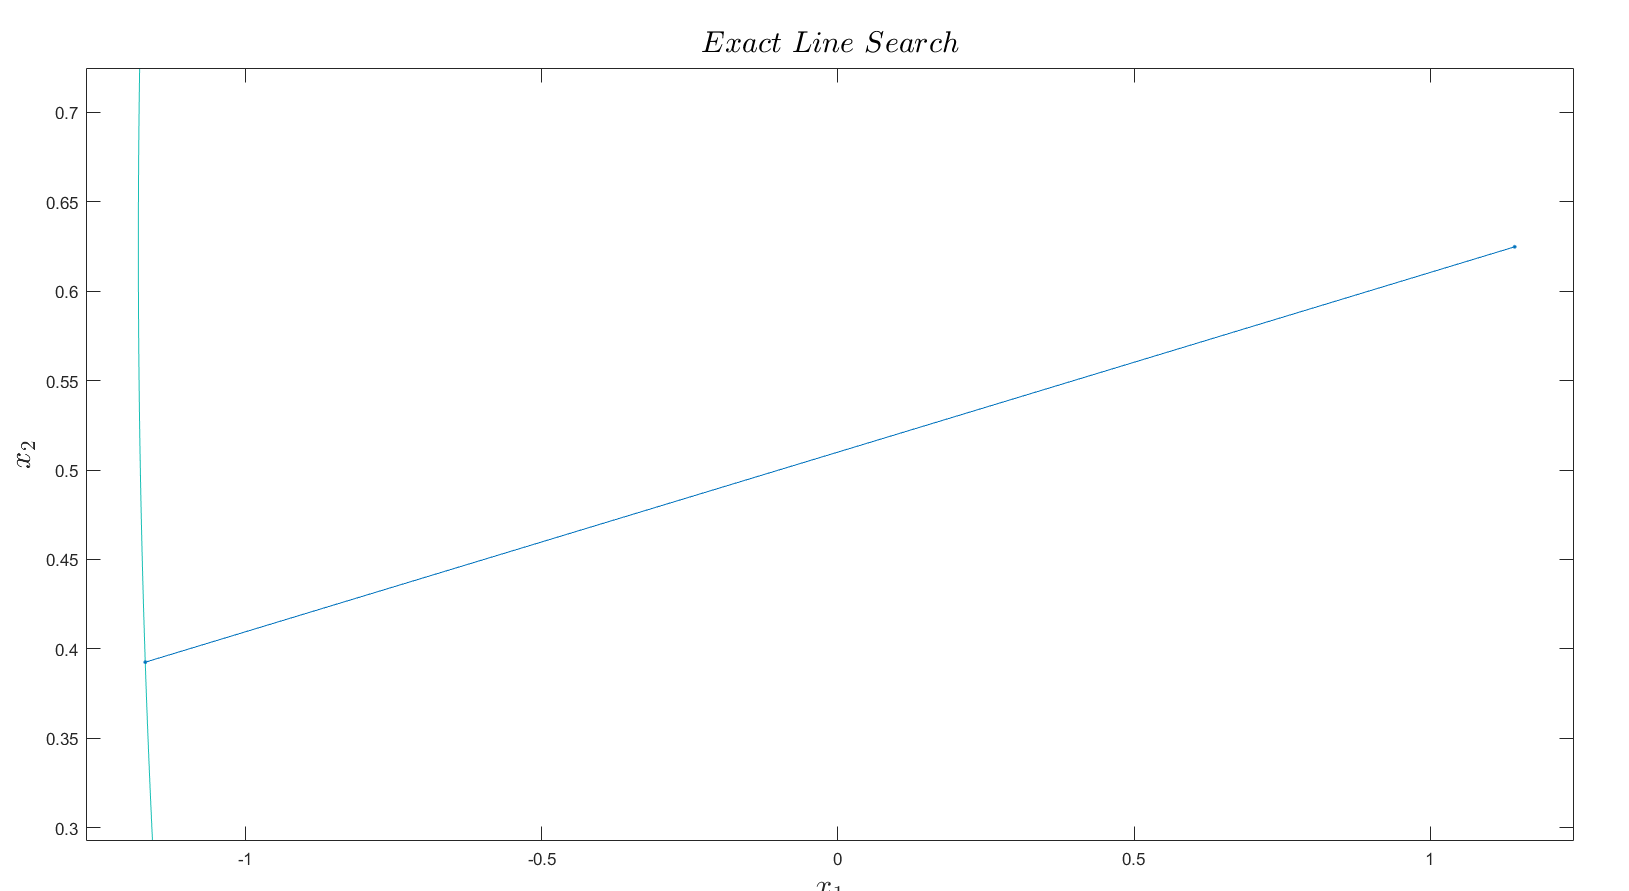
\includegraphics[width=\textwidth]{1_3.png}
				\end{subfigure}
				\hfill
				\begin{subfigure}[b]{0.45\textwidth}
					\centering
					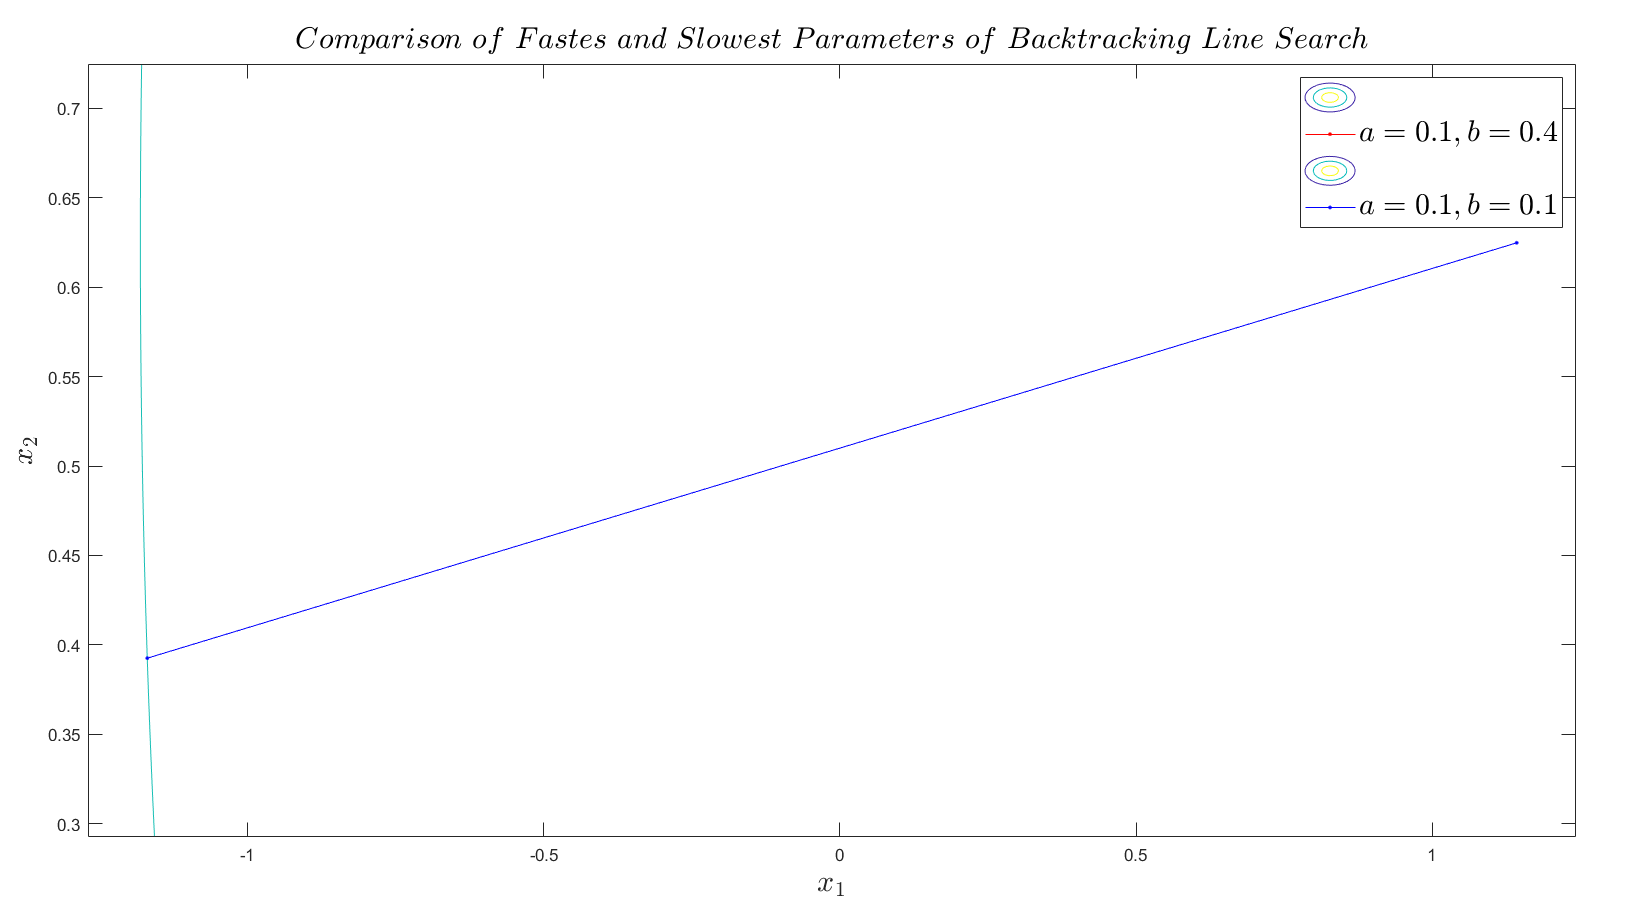
\includegraphics[width=\textwidth]{1_2.png}
				\end{subfigure}
				\caption{$\mathbb{K}=1$}
			\end{figure}
			\begin{figure}
				\centering
				\begin{subfigure}[b]{0.45\textwidth}
					\centering
					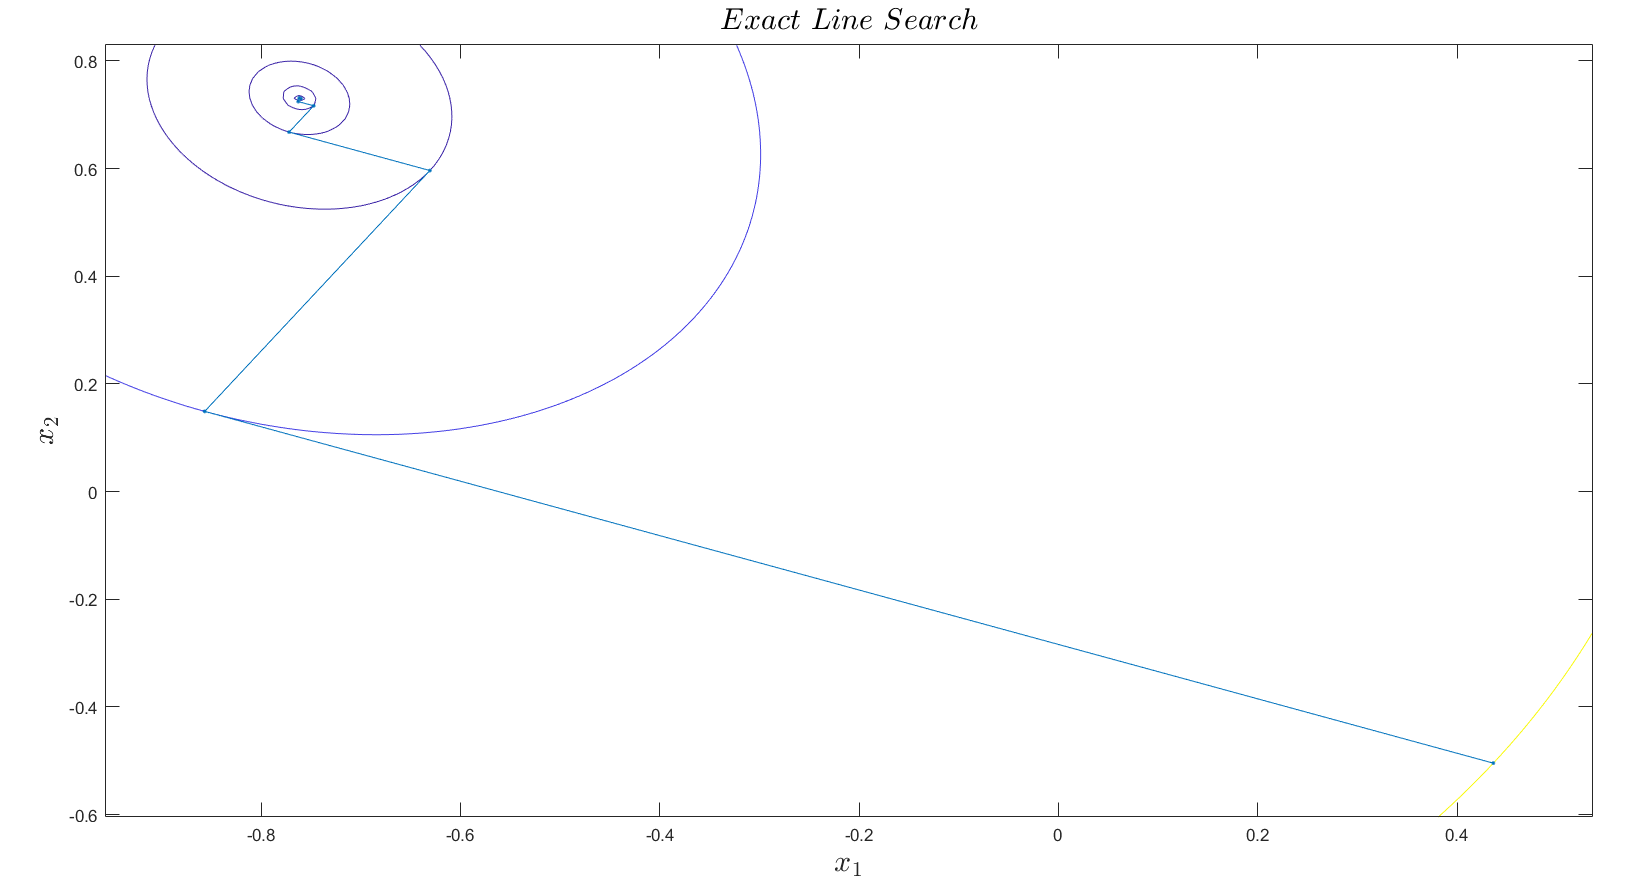
\includegraphics[width=\textwidth]{2_3.png}
				\end{subfigure}
				\hfill
				\begin{subfigure}[b]{0.45\textwidth}
					\centering
					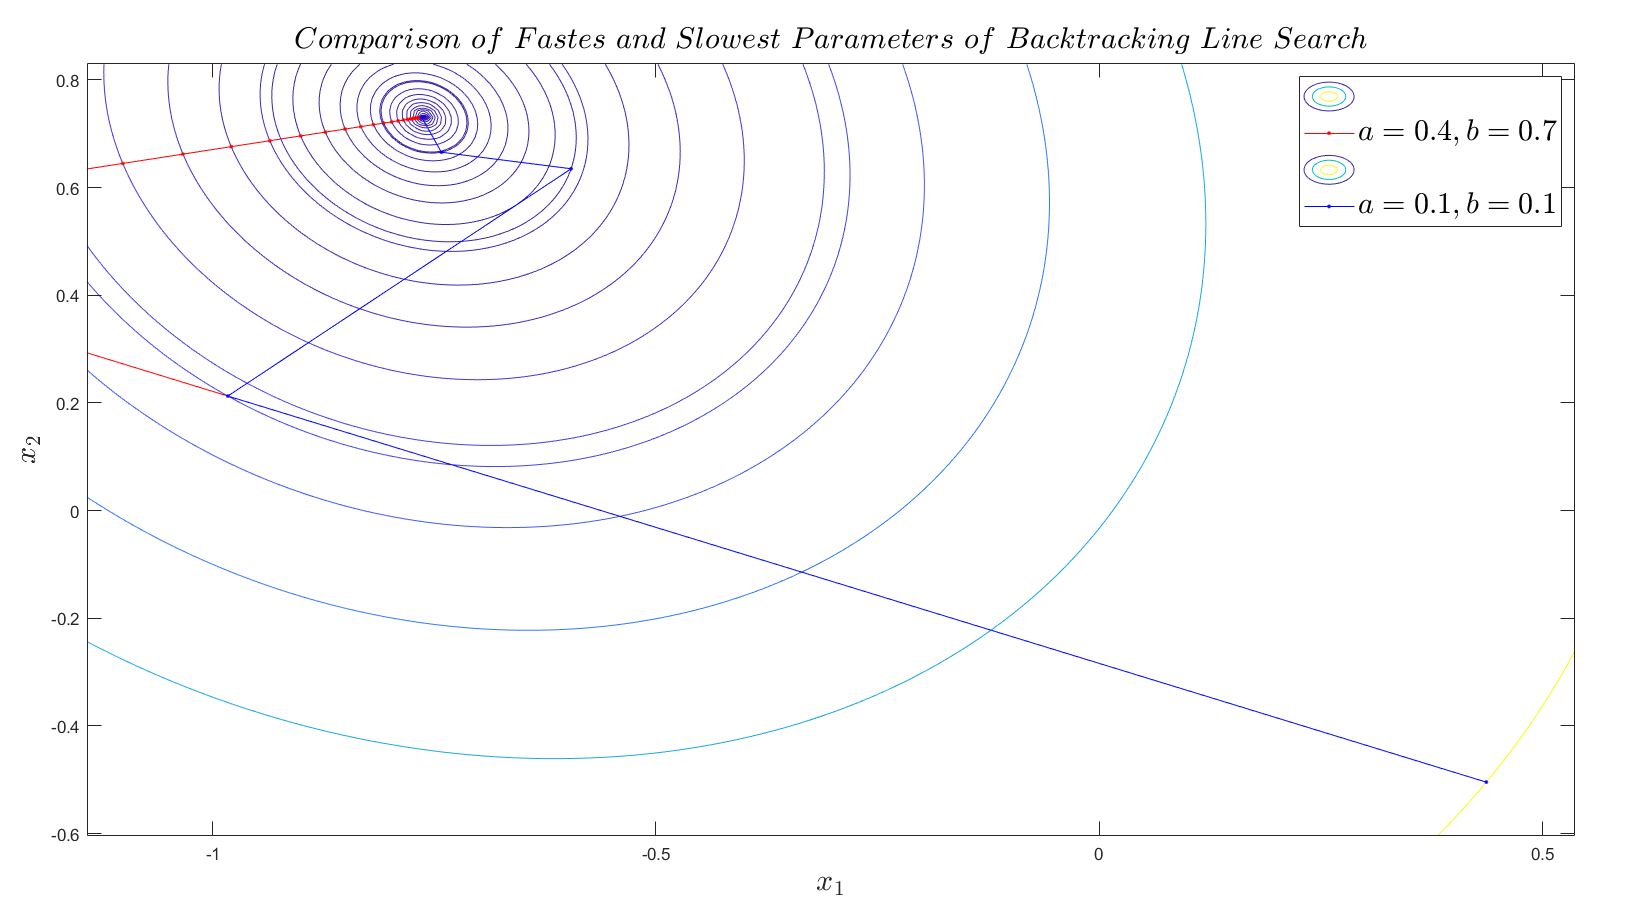
\includegraphics[width=\textwidth]{2_2.png}
				\end{subfigure}
				\caption{$\mathbb{K}=2$}
			\end{figure}
			\begin{figure}
				\centering
				\begin{subfigure}[b]{0.45\textwidth}
					\centering
					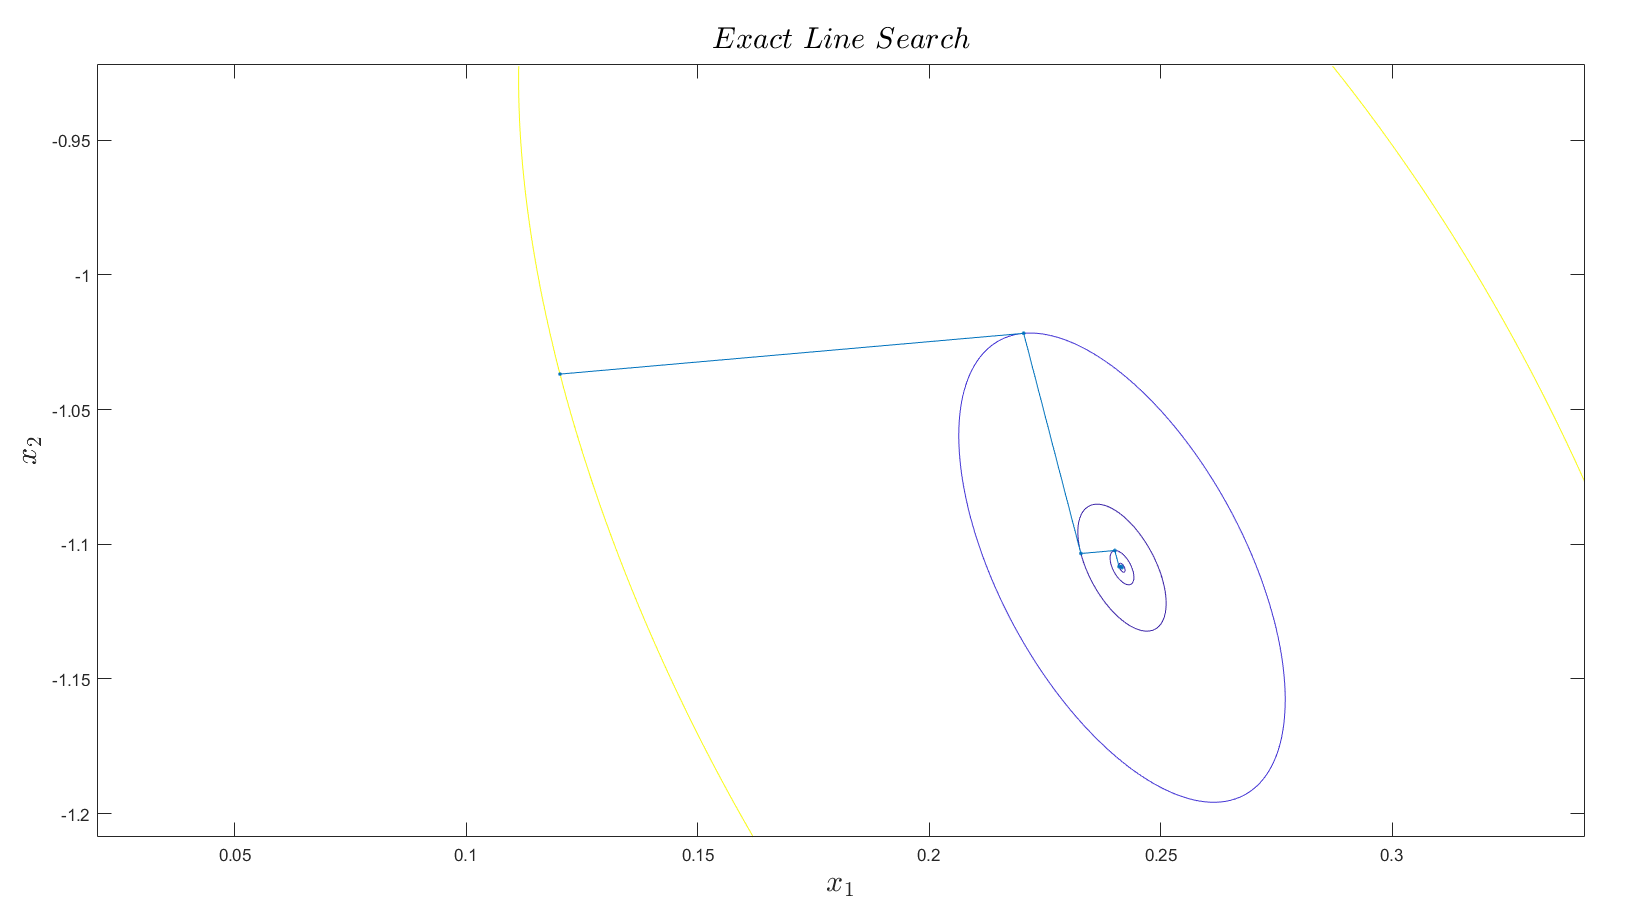
\includegraphics[width=\textwidth]{3_3.png}
				\end{subfigure}
				\hfill
				\begin{subfigure}[b]{0.45\textwidth}
					\centering
					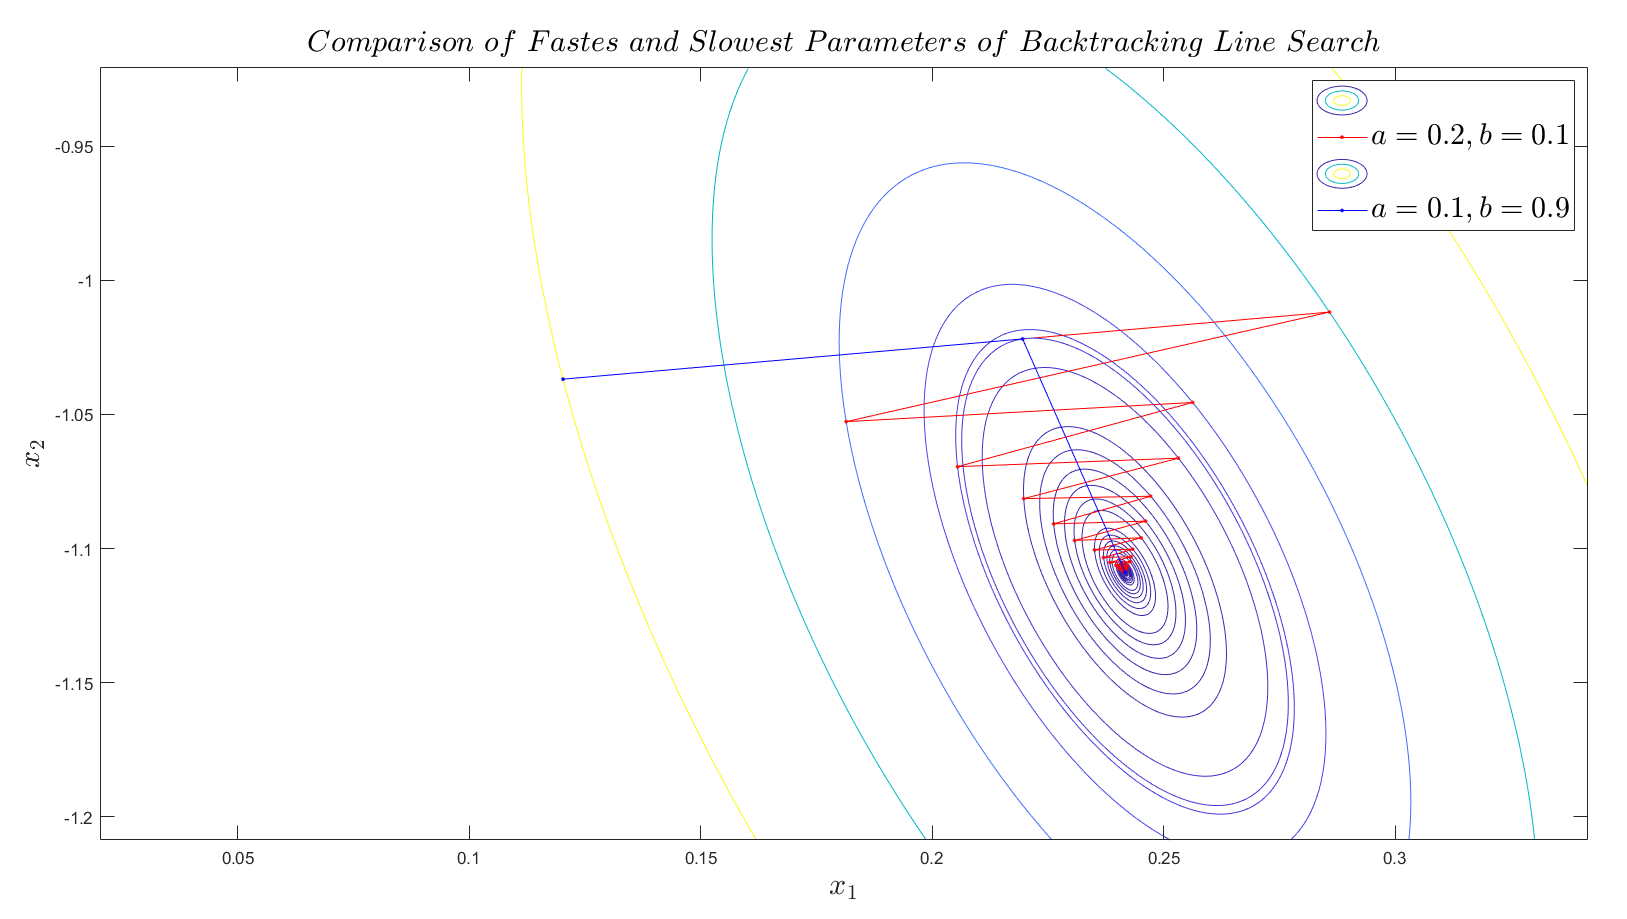
\includegraphics[width=\textwidth]{3_2.png}
				\end{subfigure}
				\caption{$\mathbb{K}=10$}
			\end{figure}
			\begin{figure}
				\centering
				\begin{subfigure}[b]{0.45\textwidth}
					\centering
					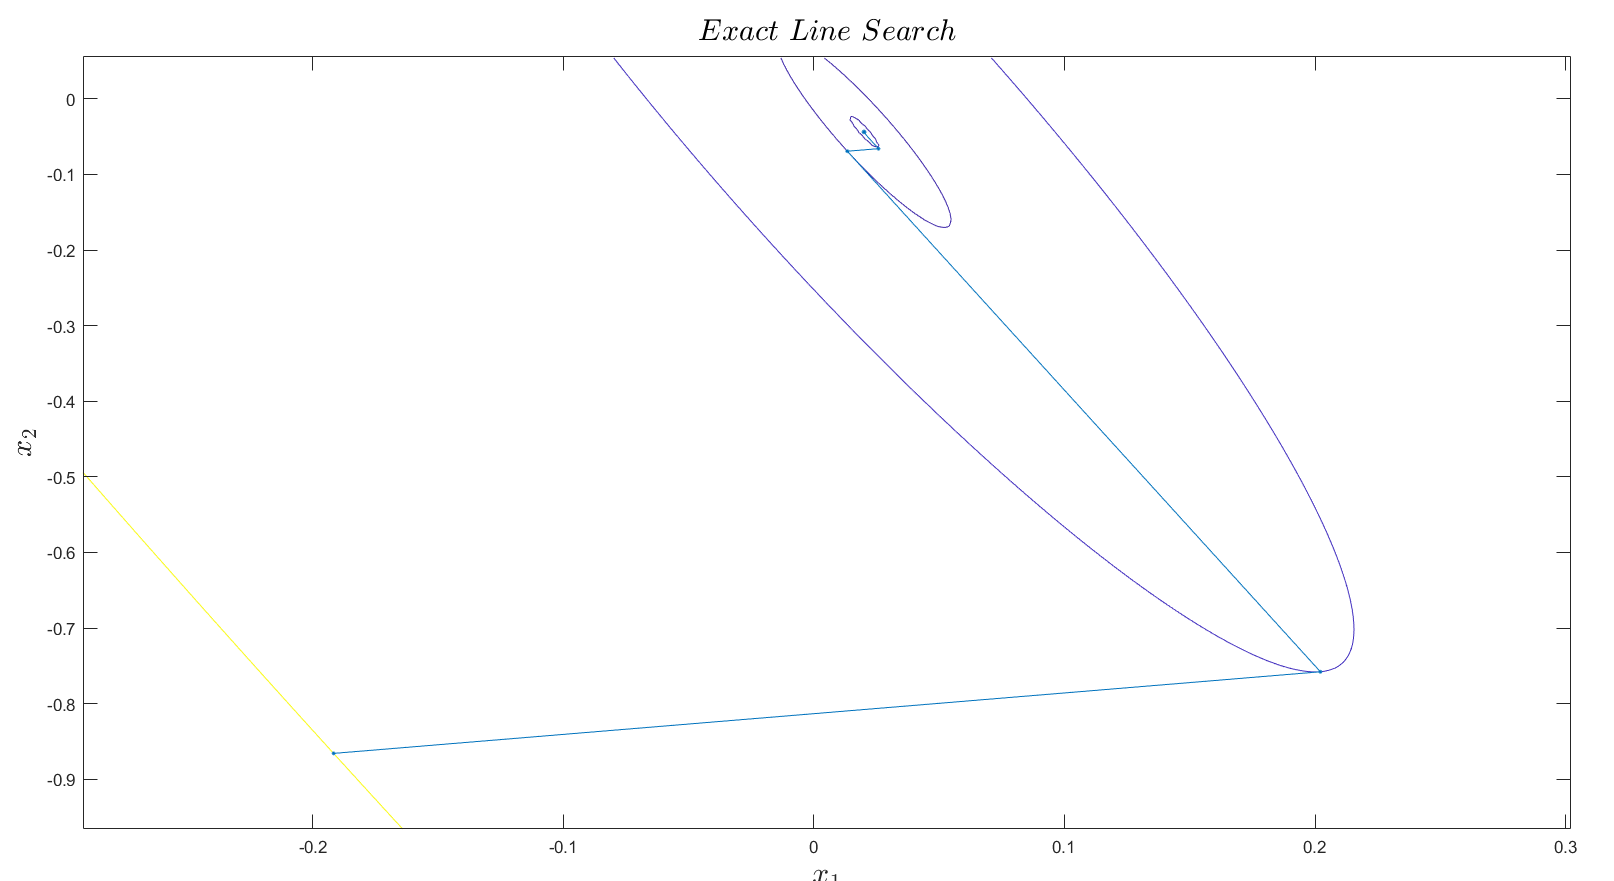
\includegraphics[width=\textwidth]{4_3.png}
				\end{subfigure}
				\hfill
				\begin{subfigure}[b]{0.45\textwidth}
					\centering
					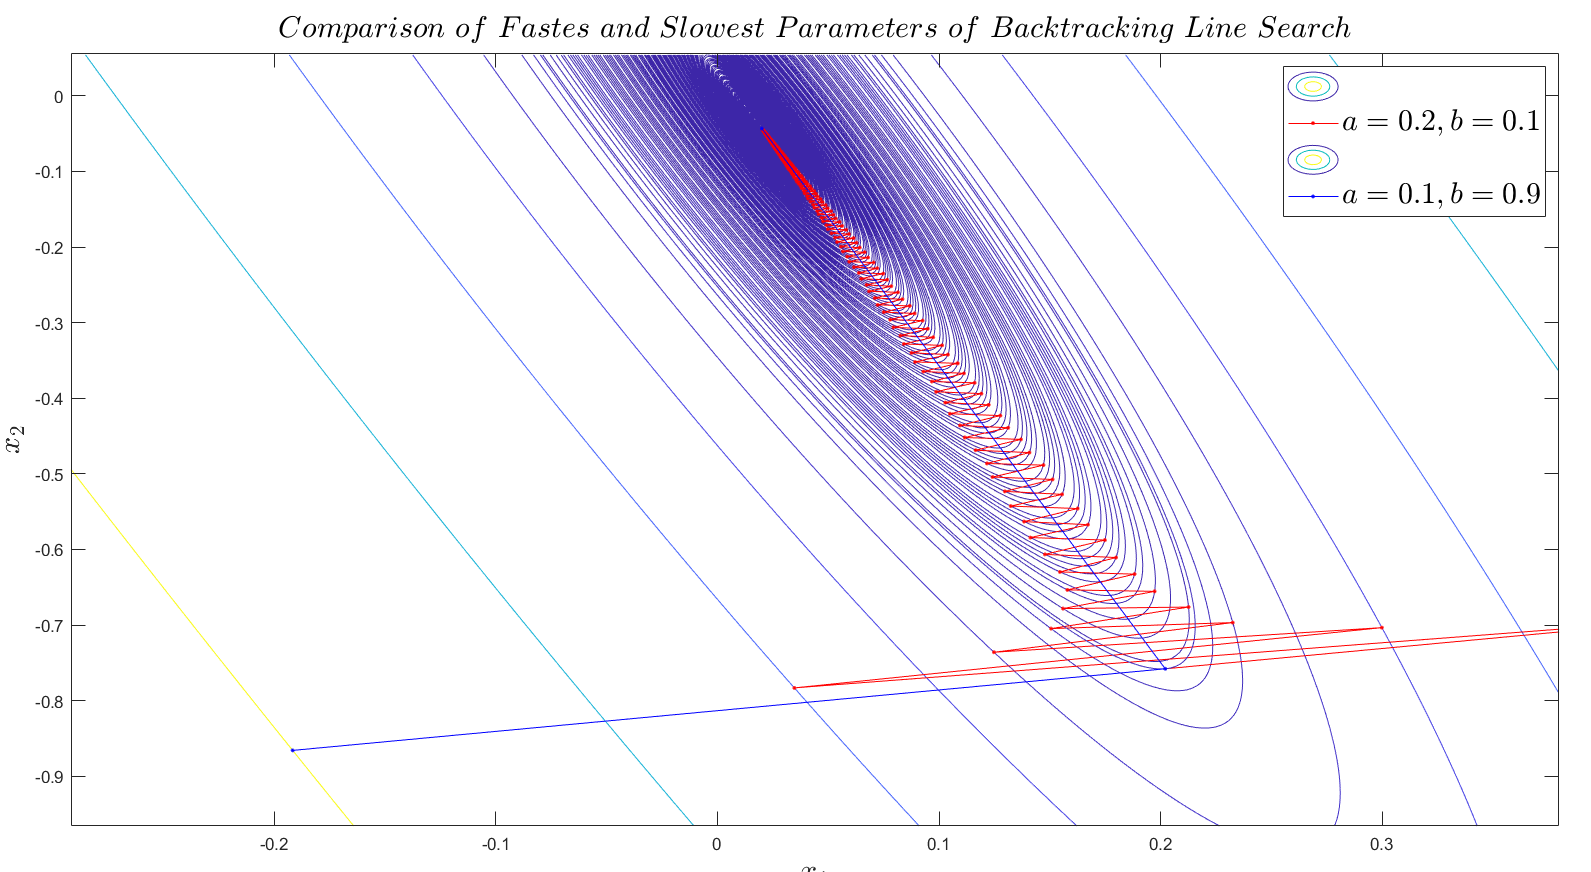
\includegraphics[width=\textwidth]{4_2.png}
				\end{subfigure}
				\caption{$\mathbb{K}=10^2$}
			\end{figure}
			\begin{figure}
				\centering
				\begin{subfigure}[b]{0.45\textwidth}
					\centering
					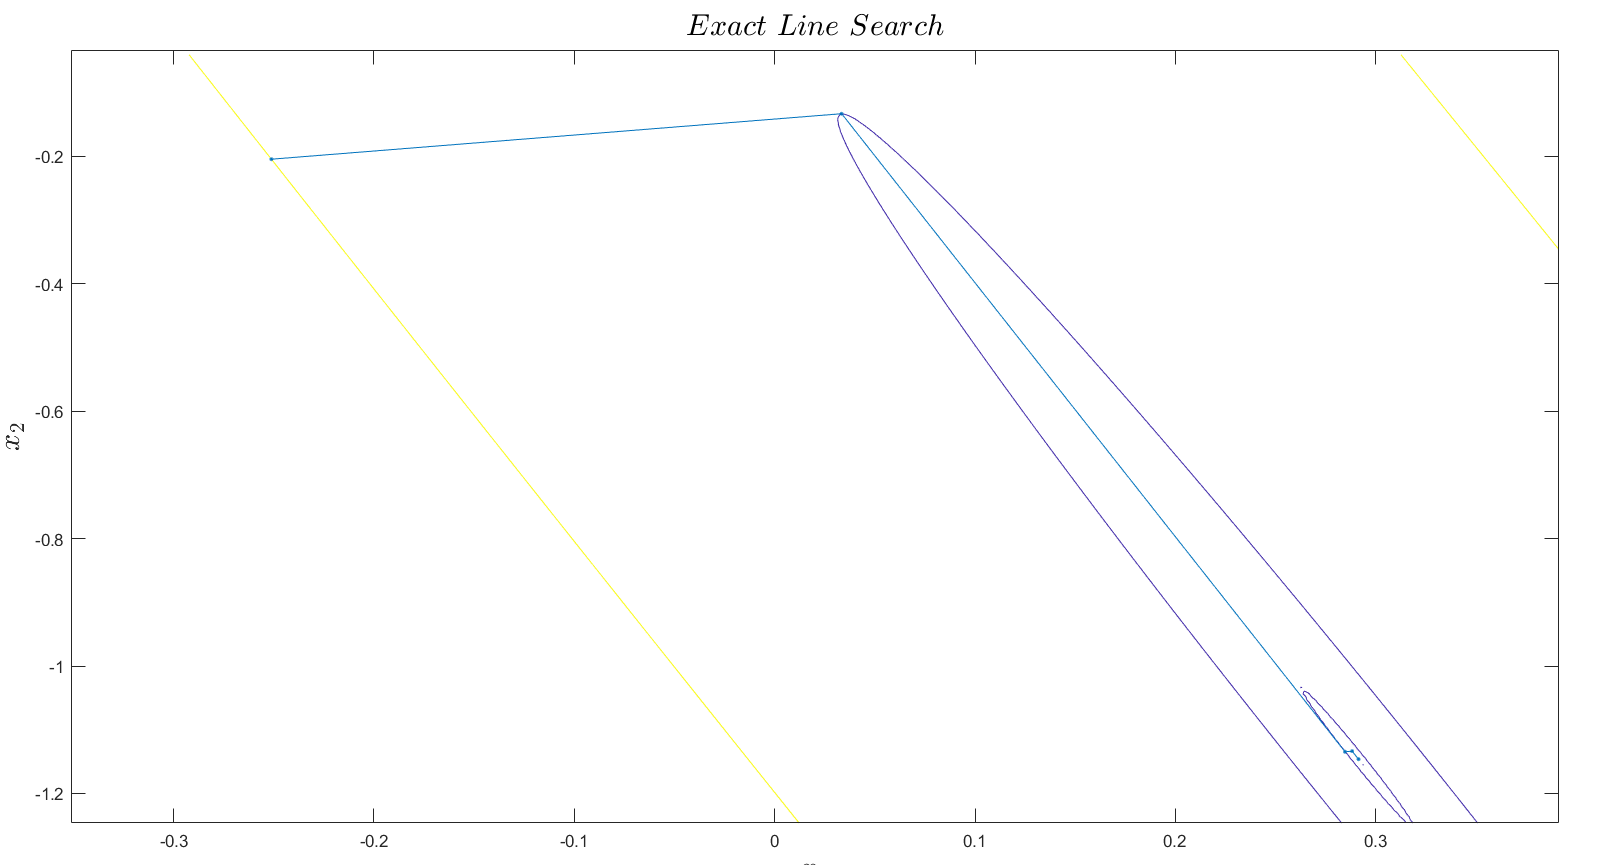
\includegraphics[width=\textwidth]{5_3.png}
				\end{subfigure}
				\hfill
				\begin{subfigure}[b]{0.45\textwidth}
					\centering
					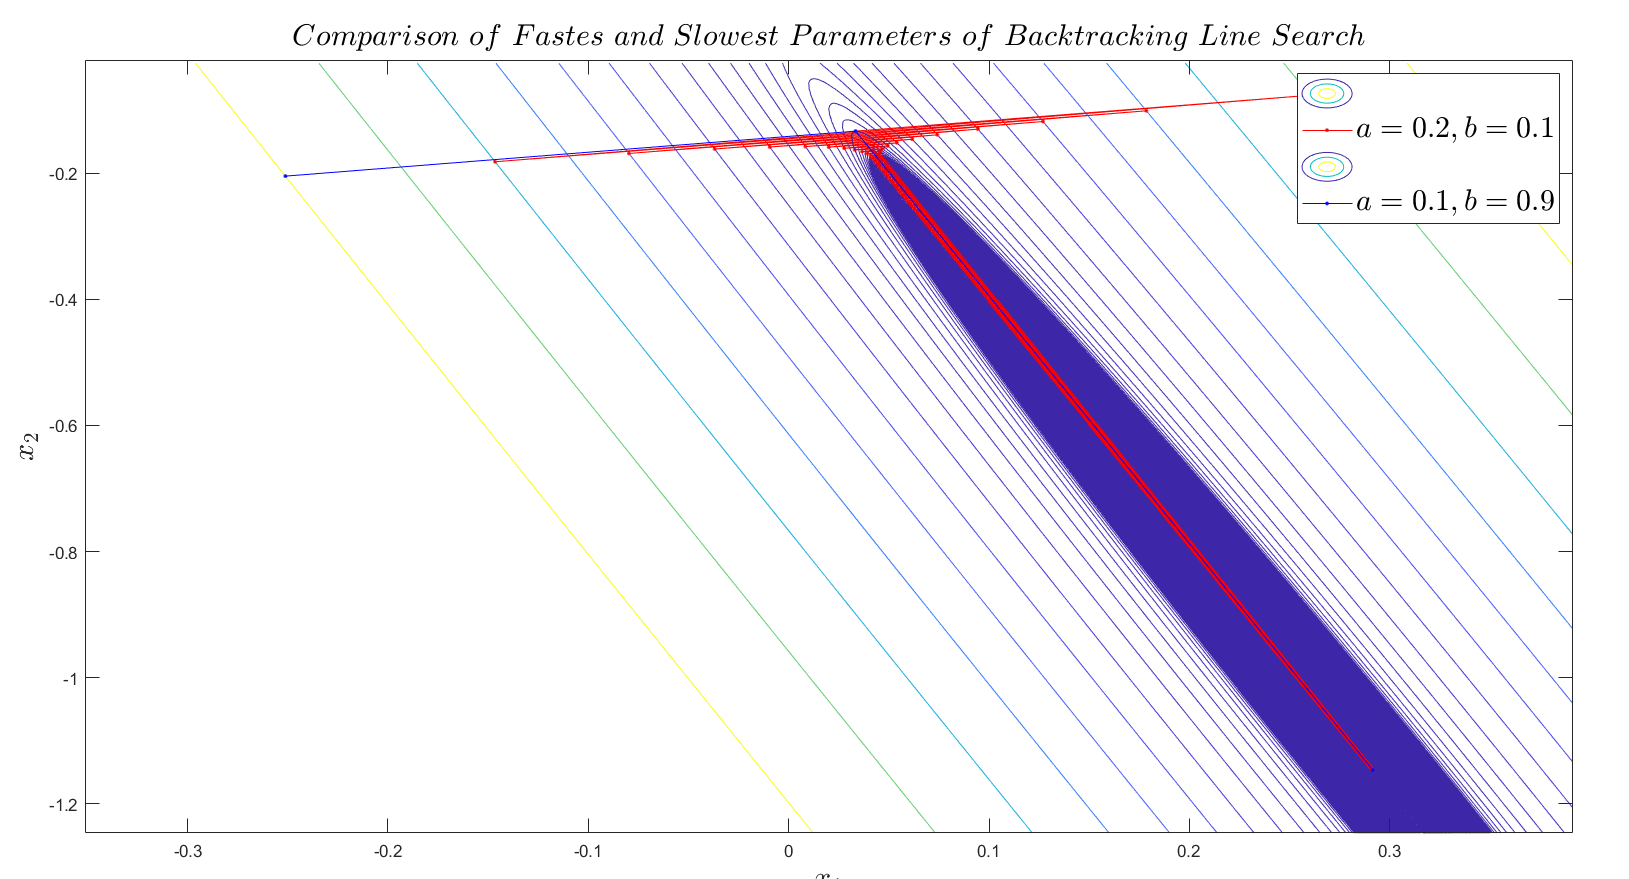
\includegraphics[width=\textwidth]{5_2.png}
				\end{subfigure}
				\caption{$\mathbb{K}=10^3$}
			\end{figure}
			In reality every $a$ and $b$ for the backtracking algorithm converges in one iteration for $\mathbb{K}=1$\\
			As $\mathbb{K}$ increases we begin to observe the zig-zag effect.\\
			We also observe that the  correct choice of the parameters $a$ and $b$ is important in order for the backtracking algorithm to converge fast.
			
			\item[vi.]
			For $\mathbb{K}=1$ the plots are empty since in one iteration the algorithms find the optimal value and hence the plots are omitted.\\
			We also observe that the slopes of each plot remain relatively the same meaning the distance from the optimal value in each iteration decreases by almost the same amount. 
			\begin{figure}
				\centering
				\begin{subfigure}[b]{0.45\textwidth}
					\centering
					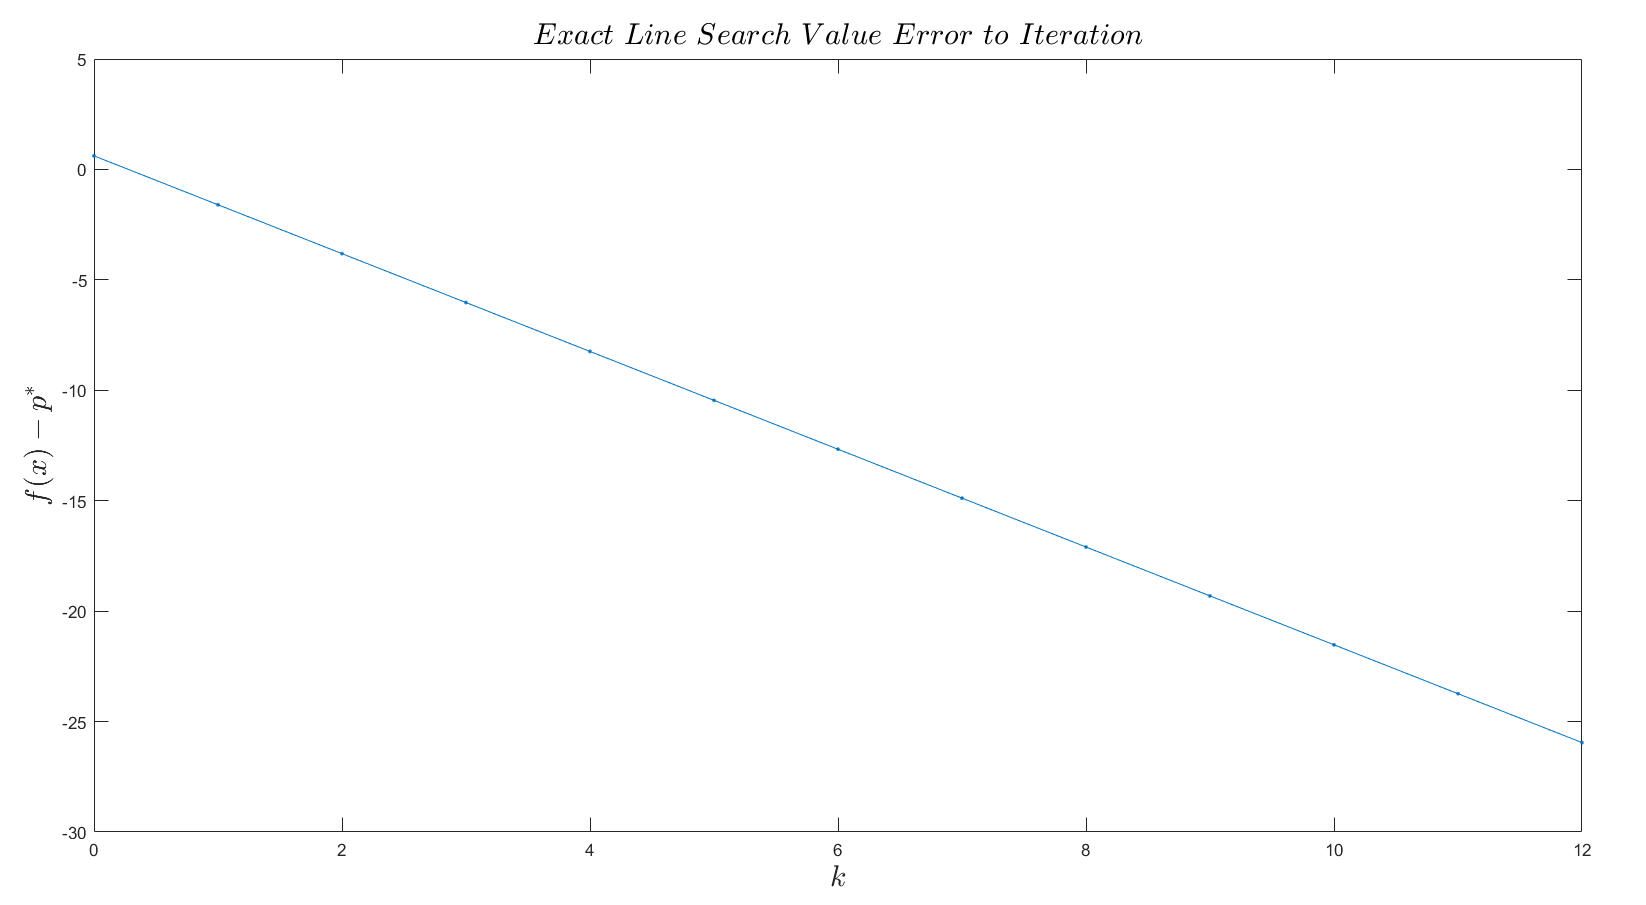
\includegraphics[width=\textwidth]{2_4.png}
				\end{subfigure}
				\hfill
				\begin{subfigure}[b]{0.45\textwidth}
					\centering
					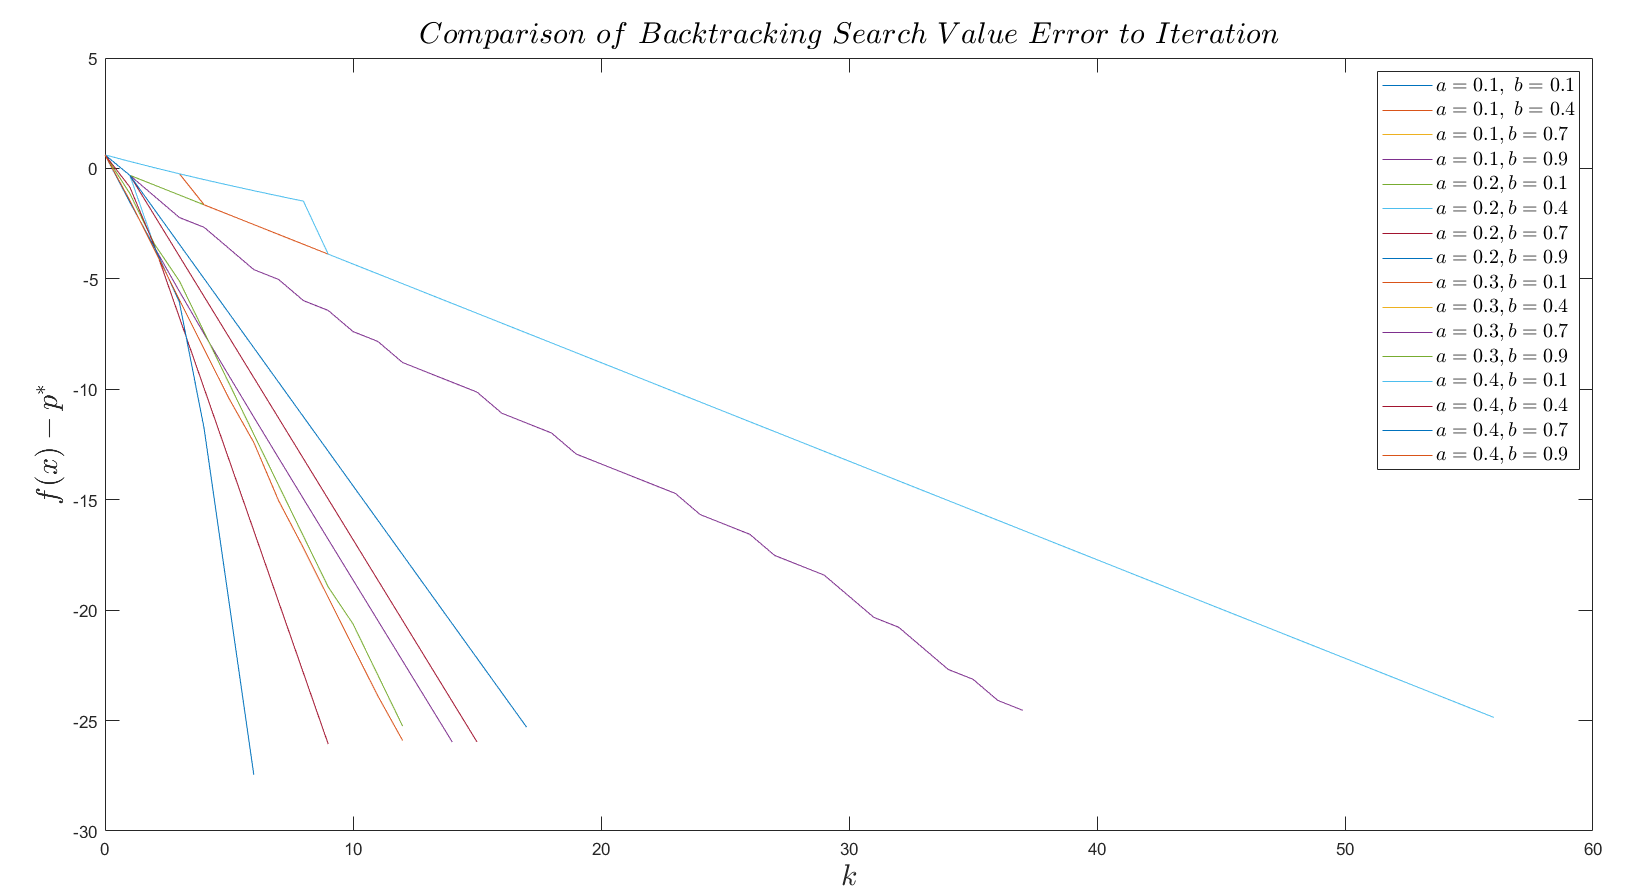
\includegraphics[width=\textwidth]{2_1.png}
				\end{subfigure}
				\caption{$\mathbb{K}=2$}
			\end{figure}
			\begin{figure}
				\centering
				\begin{subfigure}[b]{0.45\textwidth}
					\centering
					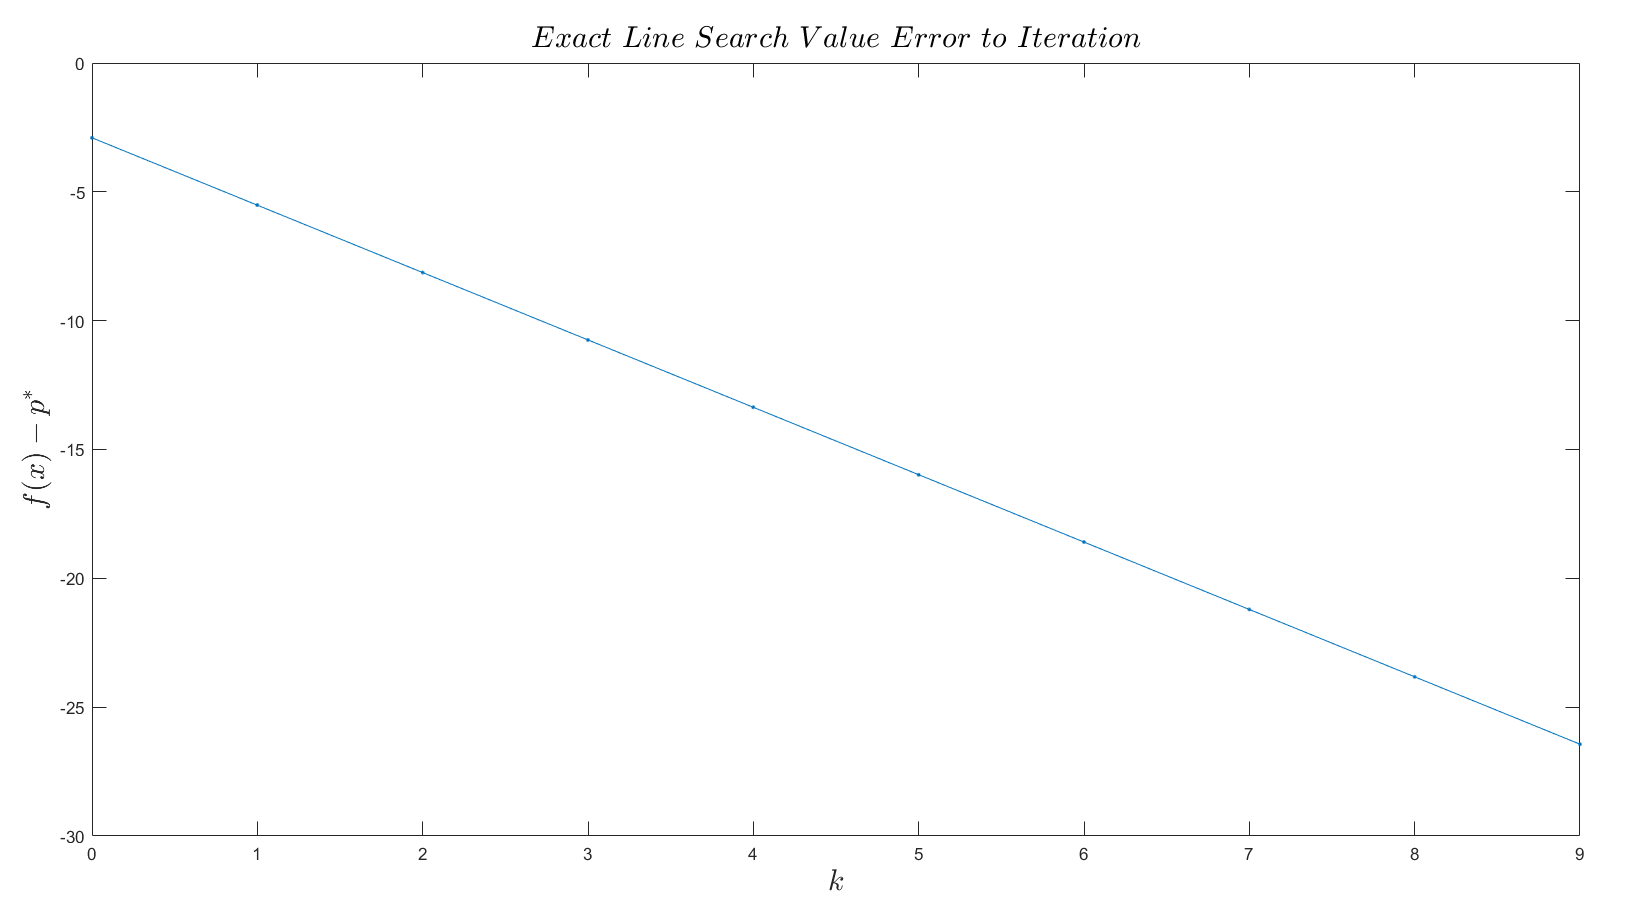
\includegraphics[width=\textwidth]{3_4.png}
				\end{subfigure}
				\hfill
				\begin{subfigure}[b]{0.45\textwidth}
					\centering
					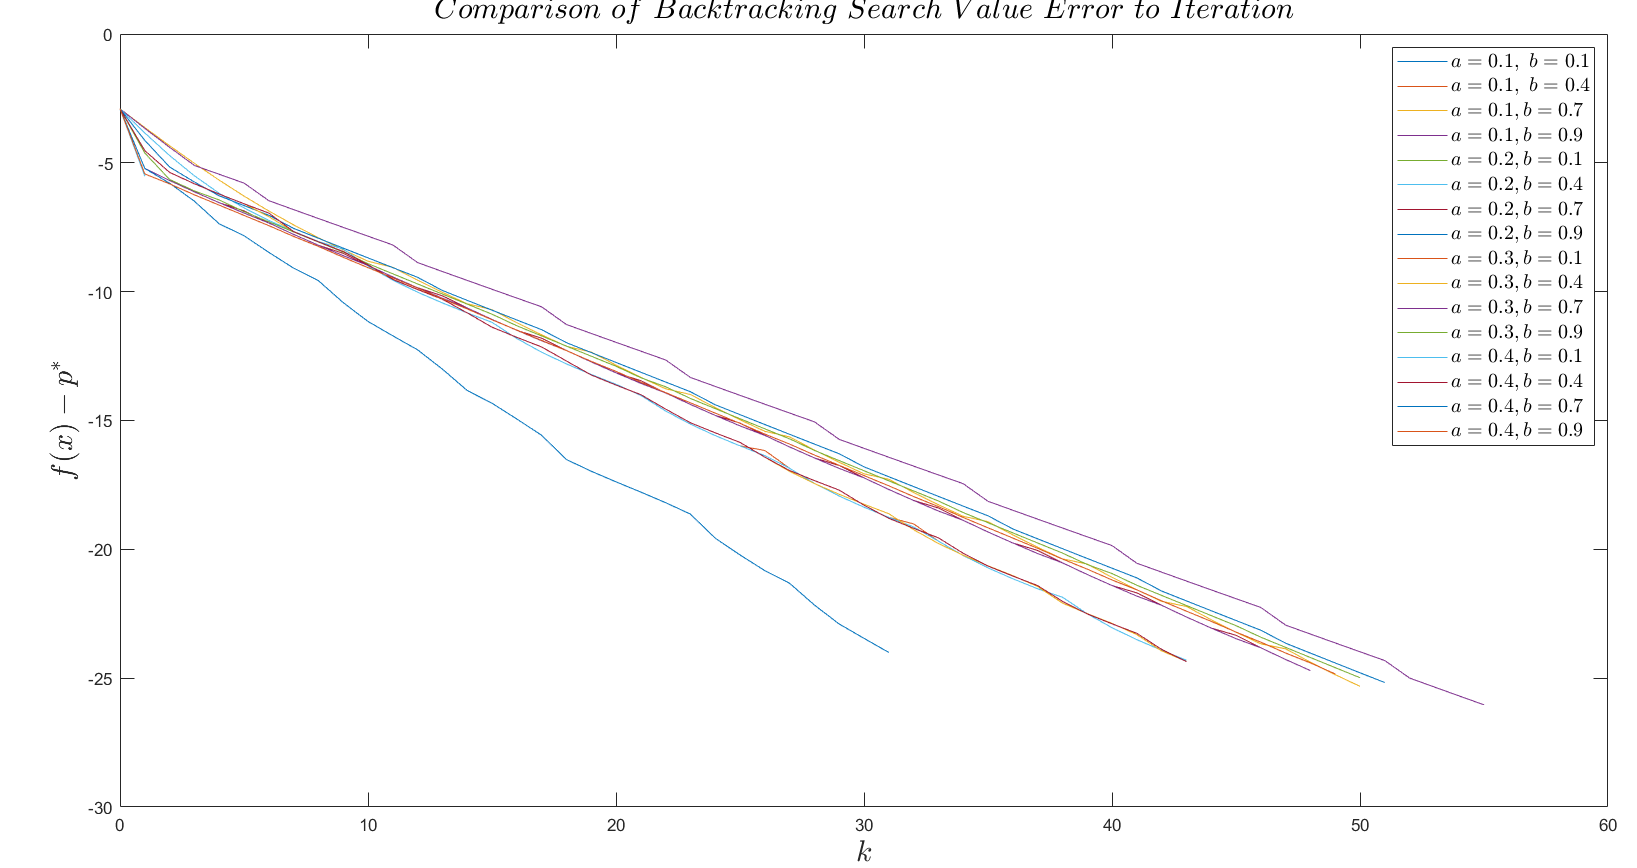
\includegraphics[width=\textwidth]{3_1.png}
				\end{subfigure}
				\caption{$\mathbb{K}=10$}
			\end{figure}
			\begin{figure}
				\centering
				\begin{subfigure}[b]{0.45\textwidth}
					\centering
					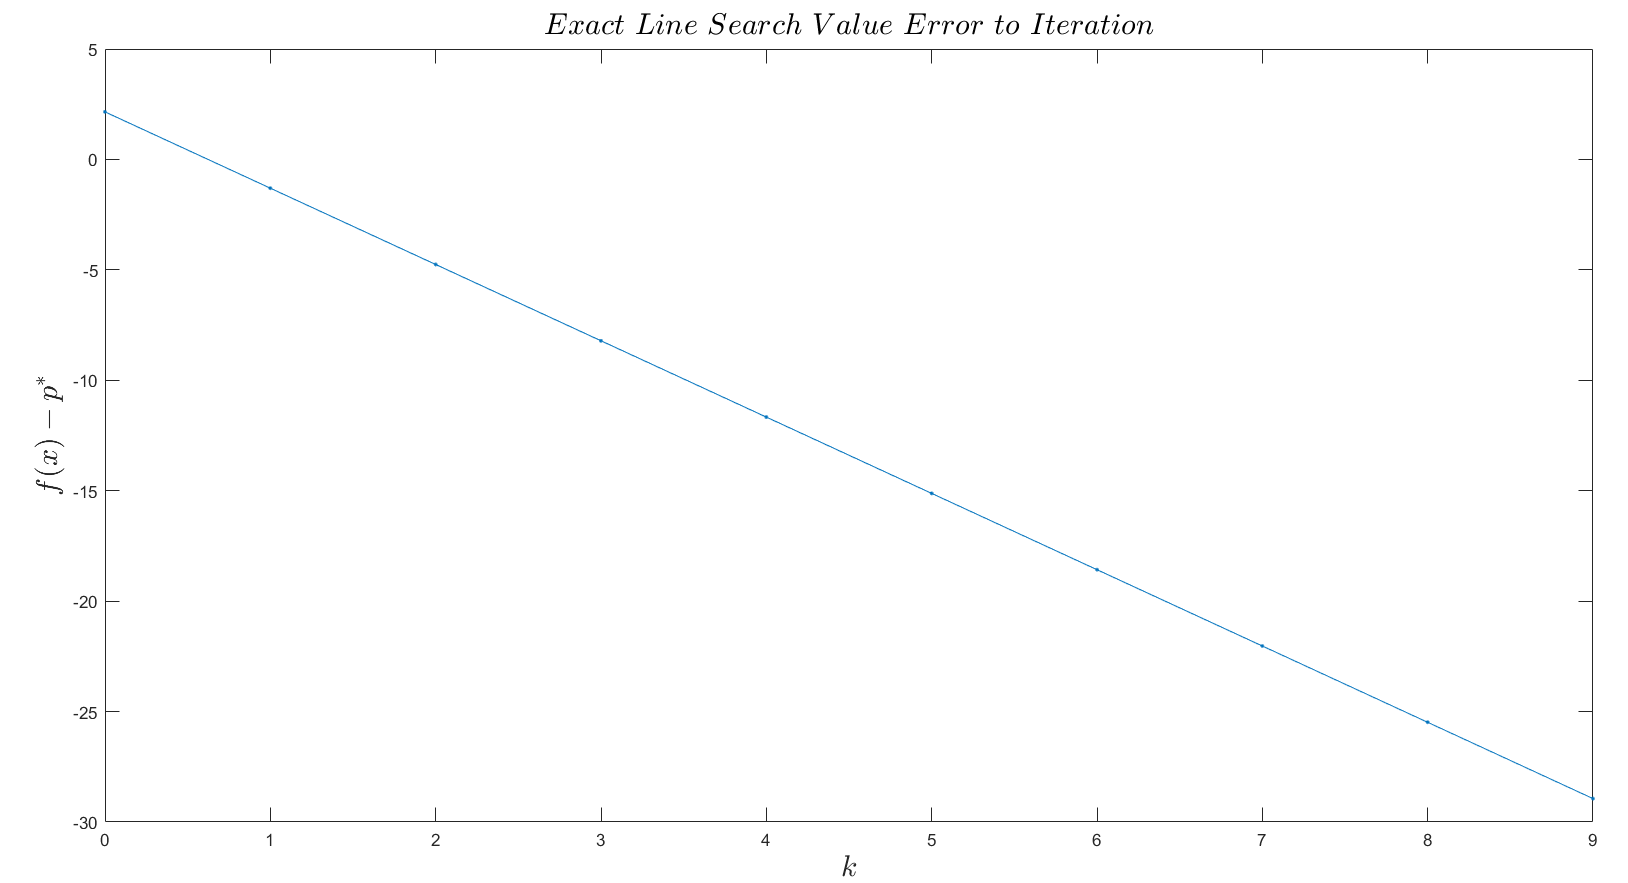
\includegraphics[width=\textwidth]{4_4.png}
				\end{subfigure}
				\hfill
				\begin{subfigure}[b]{0.45\textwidth}
					\centering
					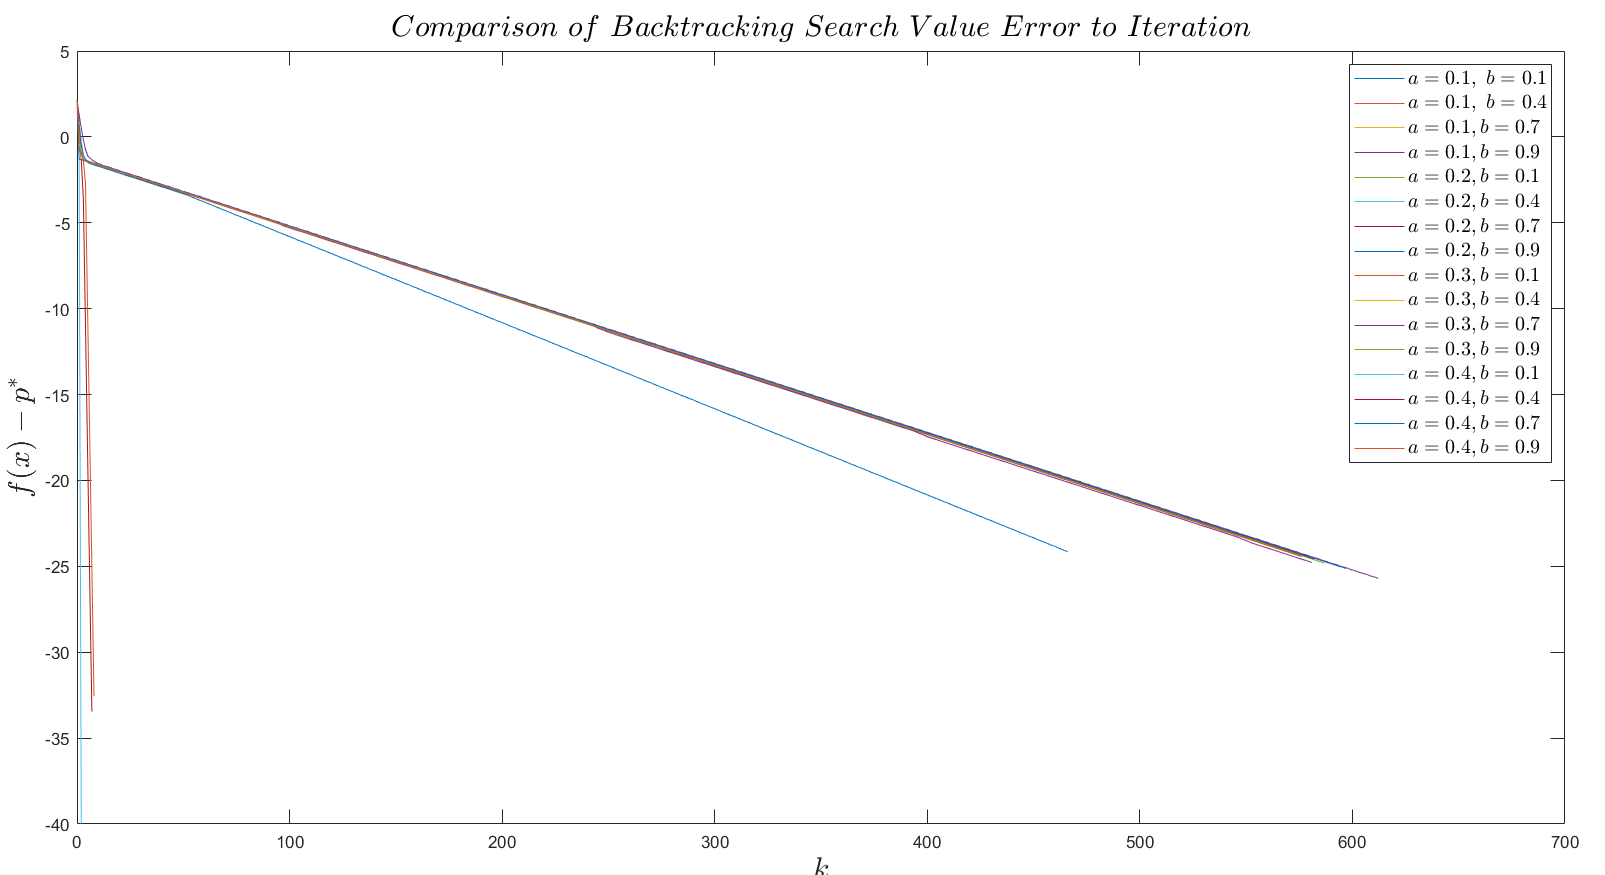
\includegraphics[width=\textwidth]{4_1.png}
				\end{subfigure}
				\caption{$\mathbb{K}=10^2$}
			\end{figure}
			\begin{figure}
				\centering
				\begin{subfigure}[b]{0.45\textwidth}
					\centering
					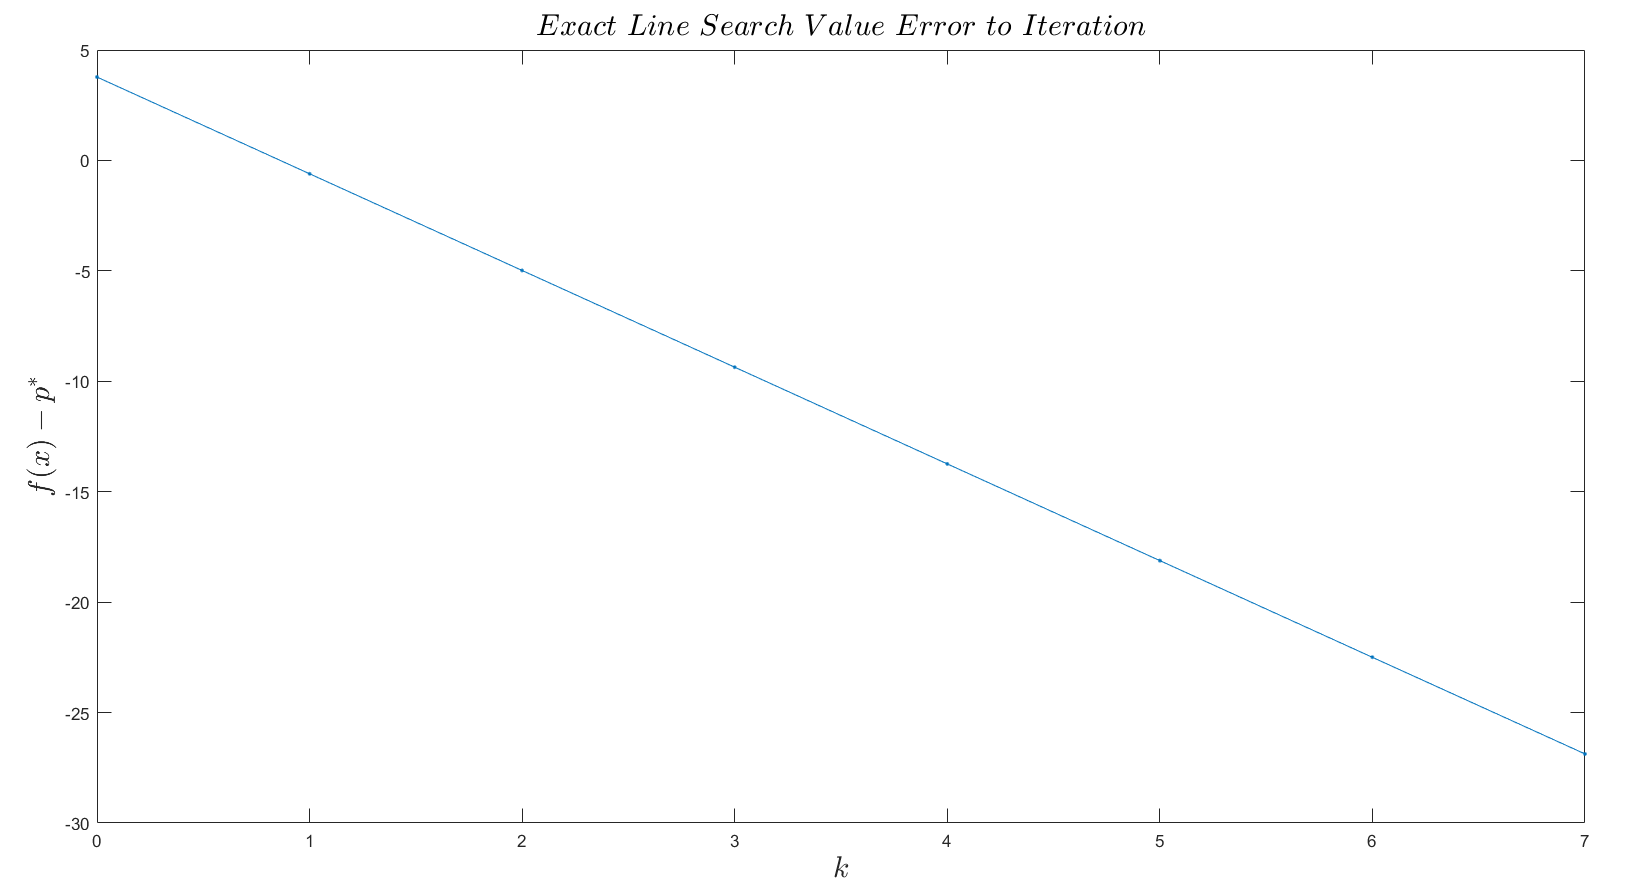
\includegraphics[width=\textwidth]{5_4.png}
				\end{subfigure}
				\hfill
				\begin{subfigure}[b]{0.45\textwidth}
					\centering
					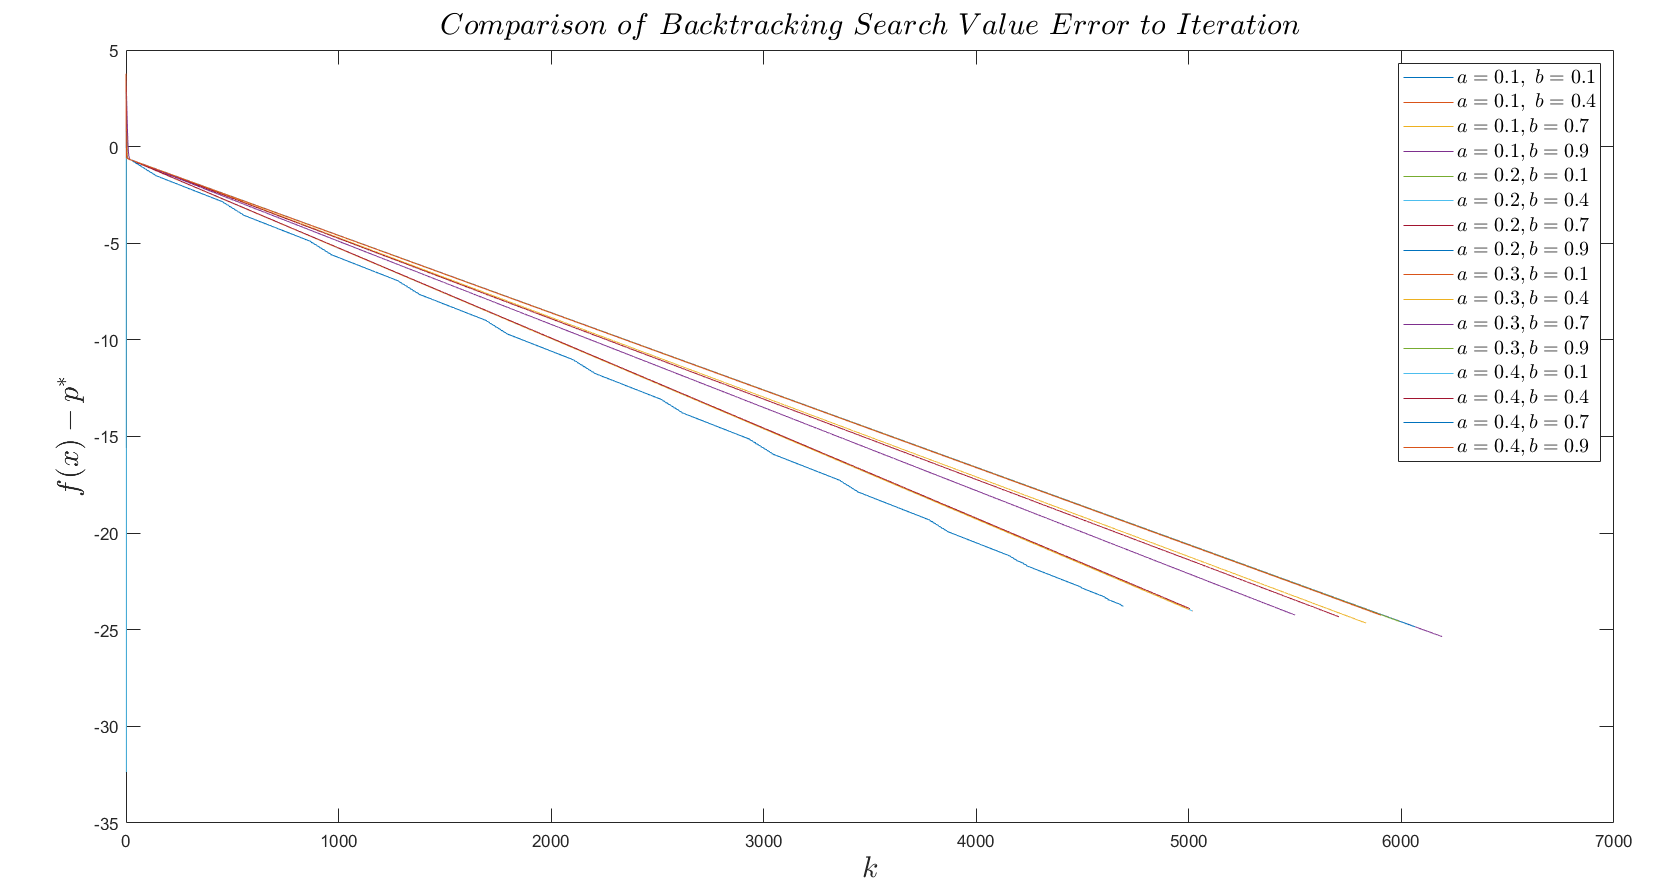
\includegraphics[width=\textwidth]{5_1.png}
				\end{subfigure}
				\caption{$\mathbb{K}=10^3$}
			\end{figure}
			\newpage
			\item[vii.]
			We have already shown that the convergence analysis for both algorithms shows that the minimum number of iterations($k_\epsilon$) that guarantees solution within accuracy $\epsilon$ : $k_\epsilon=\frac{log\big(\frac{f({\bf x_0}-{\bf p^*})}{\epsilon}\big)}{log(\frac{1}{c})}$, where $log(\frac{1}{c})=\mathbb{K}$ for the exact line search algorithm and $c\coloneqq 1- min\{2m\alpha,\frac{2\beta\alpha m}{M}\}$ for the backtracking one.
			\begin{figure}
				\centering
				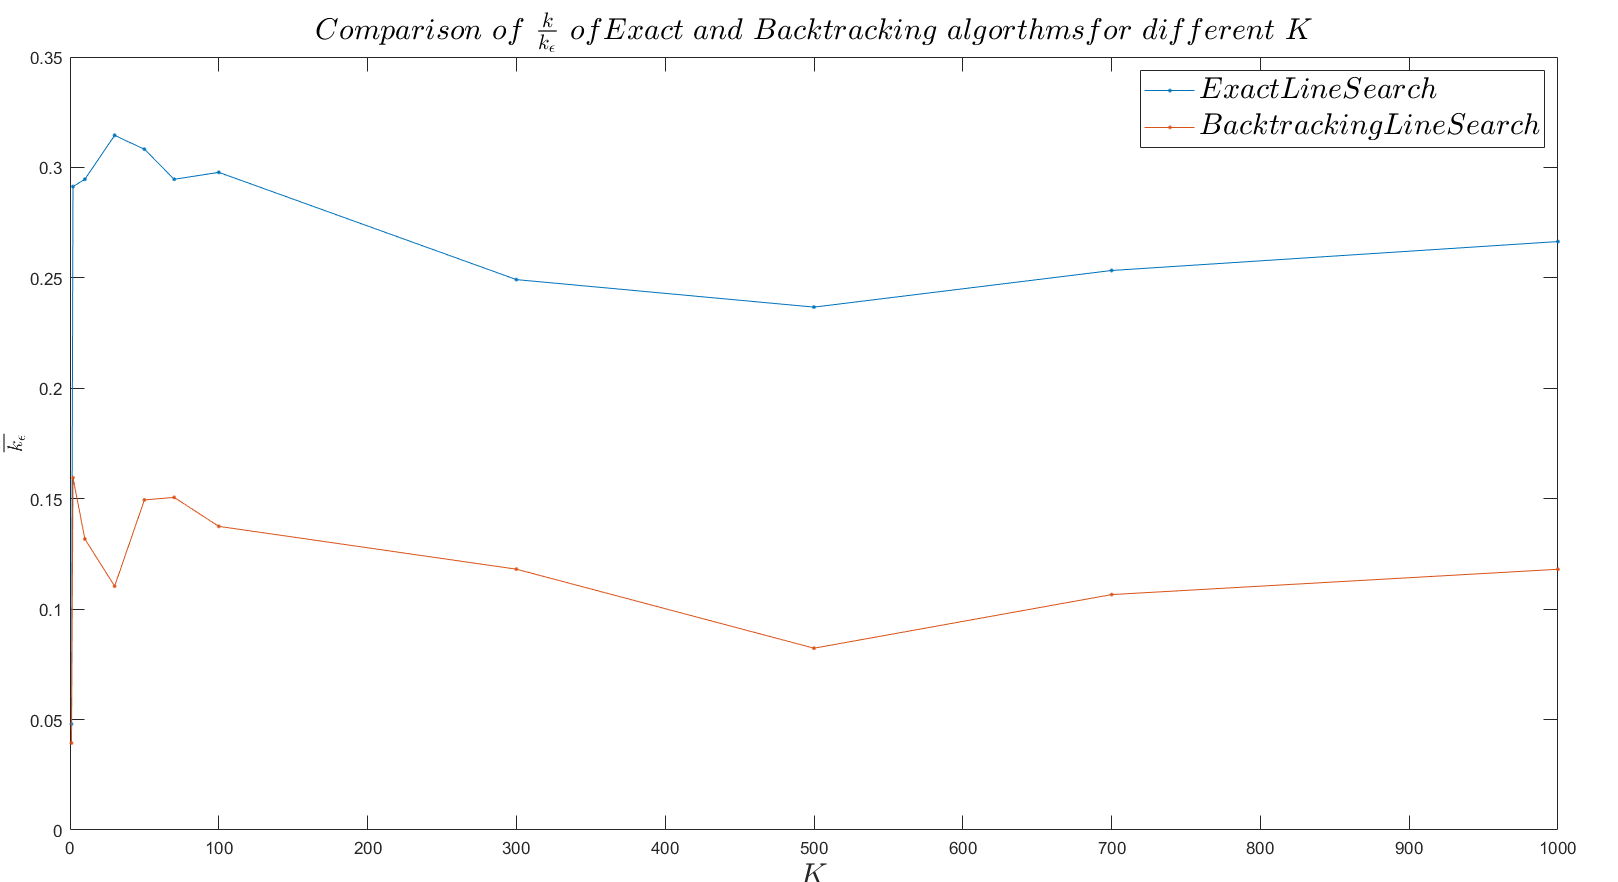
\includegraphics[width=0.9\textwidth]{6.png}
				\caption{$n=50$};
			\end{figure}
			We observe that the ratio $\frac{k}{k_\epsilon}$ for large $\mathbb{R}$ stabilizes and that the algorithms need a lot less iterations to converge than the minimum $k_\epsilon$. Also the exact line tracing algorithm converges faster than the backtracking one.
		\end{enumerate}
	\newpage
	\item[{\bf C}]
	Let ${\bf c}\in \mathbb{R}^n,{\bf b}\in\mathbb{R}^m$ and ${\bf A}\in\mathbb{R}^{mxn}$ with rows ${\bf a}_i^T,i=1,...,m$.\\
	Consider the function $f:\mathbb{R}^n\rightarrow\mathbb{R}$, defined as
	\begin{equation}
		f({\bf x})={\bf c}^T{\bf x}-\sum_{i=1}^{m}log(b_i-{\bf a}_i^T{\bf x})={\bf c}^T{\bf x}-sum(log({\bf b}-{\bf Ax}))
	\end{equation}
	with $x\in\mathbb{R}^n$ and $m>n$(or $m>>n$).
	\begin{itemize}
		\item The set ${\bf dom}f$ contains only the points ${\bf x\in \mathbb{R}^n}$ for which the arguments of the logarithms are positive.
		\begin{enumerate}
			\item 
			Let $x_1,x_2\in {dom}f \Rightarrow {\bf b}-{\bf Ax_1}>0$ and ${\bf b}-{\bf Ax_2}>0$ \\
			Let $0<\theta<1$:
			\begin{equation}
				\begin{split}
					\begin{rcases}
						{\bf b}-{\bf A}{\bf x_1}>0 \iff \theta{\bf b}-\theta{\bf A}{\bf x_1}>0 \\
						{\bf b}-{\bf A}{\bf x_1}>0 \iff (1-\theta){\bf b}-(1-\theta){\bf A}{\bf x_1}>0
					\end{rcases}\iff \\
				 	\theta{\bf b}-\theta{\bf A}{\bf x_1}+(1-\theta){\bf b}-(1-\theta){\bf A}{\bf x_1}>0 \iff {\bf b}-{\bf A}(\theta{\bf x_1+(1-\theta){\bf x_2}})<0
				\end{split}
			\end{equation}
			Therefore ${\bf dom}f$ is convex.
			
			\item
			Let $x_1,x_2\in {dom}f$ and $0<\theta<1$:\\
			The $\nabla f({\bf x})$:
			\begin{equation}
				\begin{split}
				 	\nabla f({\bf x})&=\nabla{\bf c}^T{\bf x}-\sum_{j=1}^{m}\nabla log(b_j-{\bf a}_j^T{\bf x})\\
				 	&=c-\sum_{i=1}^{m}\frac{\nabla({\bf a}_i^T{\bf x})}{(b_i-{\bf a}_i^T{\bf x}}\\
				 	&=c-\sum_{i=1}^{m}\frac{{\bf a}_i}{b_i-{\bf a}_i^T{\bf x}}
				\end{split}
			\end{equation}
			The $\nabla^2 f({\bf x})$ using the chain rule for calculating the hessian:
			\begin{equation}
				\begin{split}
					\nabla^2 f({\bf x})&=\nabla^2 ({\bf c}^T{\bf x})-\sum_{i=1}^{m}\nabla^2log(b_i-{\bf a}_i^T{\bf x})\\
					&=-\sum_{i=1}^{m}\frac{1}{b_i-{\bf a}_i^T{\bf x}}\nabla^2(b_i-{\bf a}_i^T{\bf x})-\frac{1}{(b_i-{\bf a}_i^T{\bf x})^2}\nabla(b_i-{\bf a}_i^T{\bf x})\nabla^T(b_i-{\bf a}_i^T{\bf x})\\
					&=\sum_{i=1}^{m}\frac{{\bf a}_i{\bf a}_i^T}{(b_i-{\bf a}_i^T{\bf x})^2}
				\end{split}
			\end{equation}
			If the $\nabla^2 f({\bf x})$ is positive definite then $f$ is convex.\\
			Let $z\in\mathbb{R}^m$:
			\begin{equation}
				\begin{split}
					{\bf z}^T\nabla^2f({\bf x}){\bf z}&={\bf z}^T\big(\sum_{i=1}^{m}\frac{{\bf a}_i{\bf a}_i^T}{(b_i-{\bf a}_i^T{\bf x})^2}\big){\bf z}=\sum_{i=1}^{m}\frac{{\bf z}^T{\bf a}_i{\bf a}_i^T{\bf z}}{(b_i-{\bf a}_i^T{\bf x})^2}\\
					&=\sum_{i=1}^{m}\frac{({\bf a}_i^T{\bf z})^T{\bf a}_i^T{\bf z}}{(b_i-{\bf a}_i^T{\bf x})^2}\\
					&=\sum_{i=1}^{m}\frac{||{\bf a}_i^T{\bf z}||_2^2}{(b_i-{\bf a}_i^T{\bf x})^2}>0\forall{\bf z}\in\mathbb{R}^m-\{{\bf 0}\}
				\end{split}
			\end{equation}
			Therefore $\nabla^2 f({\bf x})$ is positive definite and $f$ is convex.
		\end{enumerate}
	\end{itemize}
	\begin{enumerate}
		\item[a]
		We minimize $f$ using cvx:\\
		{\bf Code}:
		\lstinputlisting[firstline=13, lastline=18]{Exercise2_C.m}
		\newpage
		\item[b]
		\begin{figure}
			\centering
			\begin{subfigure}[b]{0.45\textwidth}
				\centering
				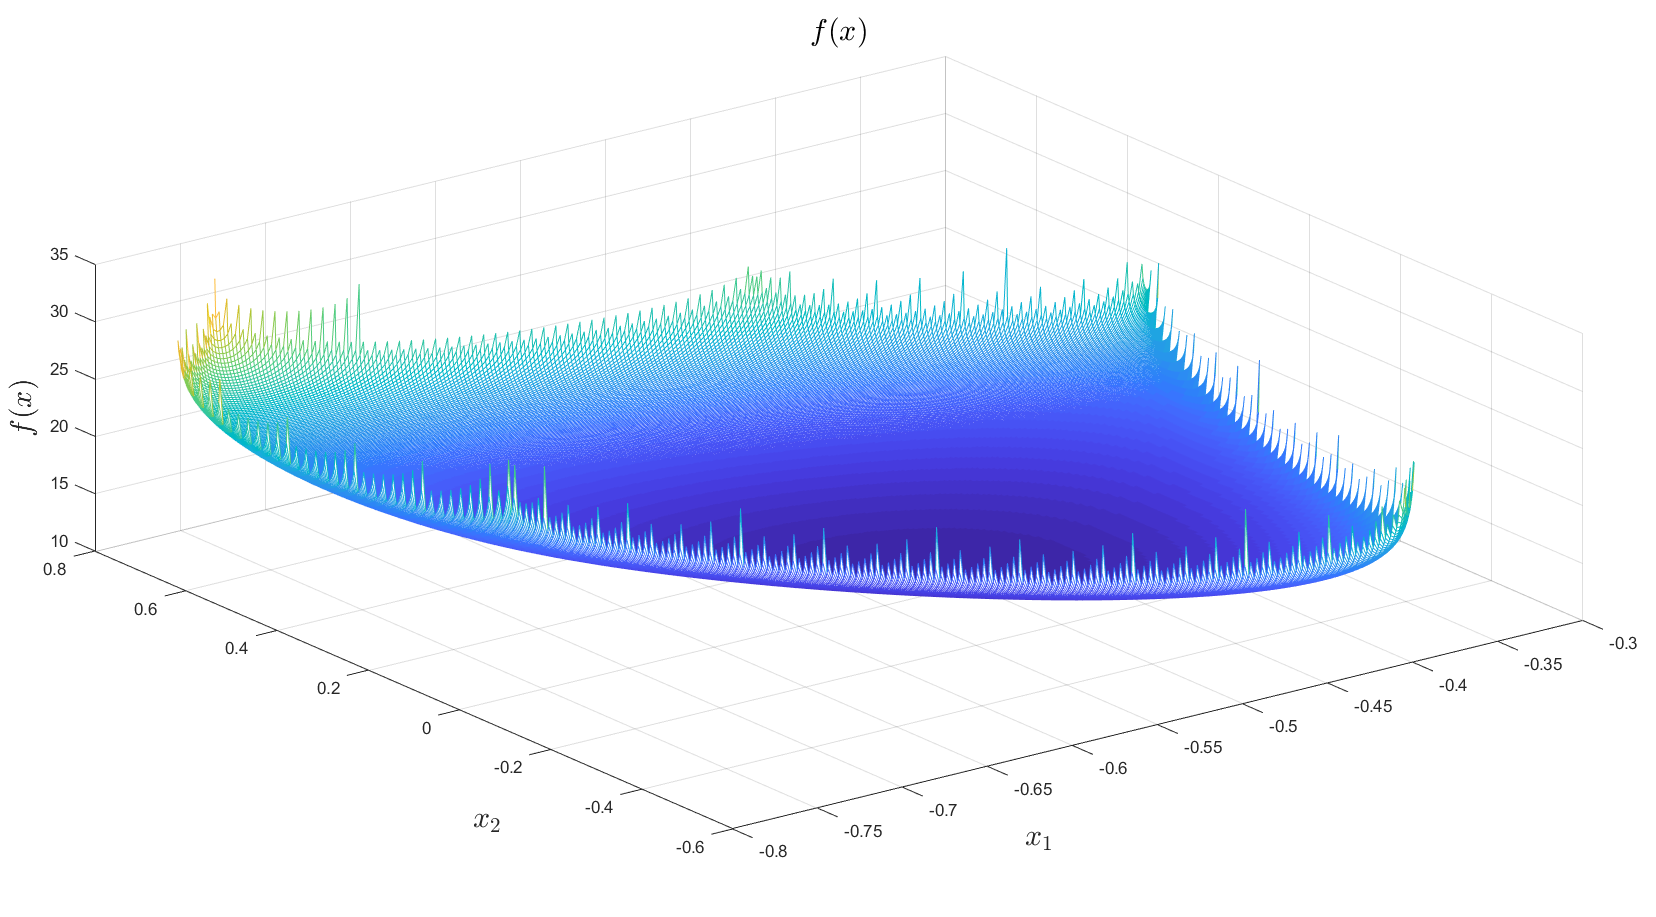
\includegraphics[width=\textwidth]{C_b_1.png}
				\caption{Plot of $f$}
			\end{subfigure}
			\hfill
			\begin{subfigure}[b]{0.45\textwidth}
				\centering
				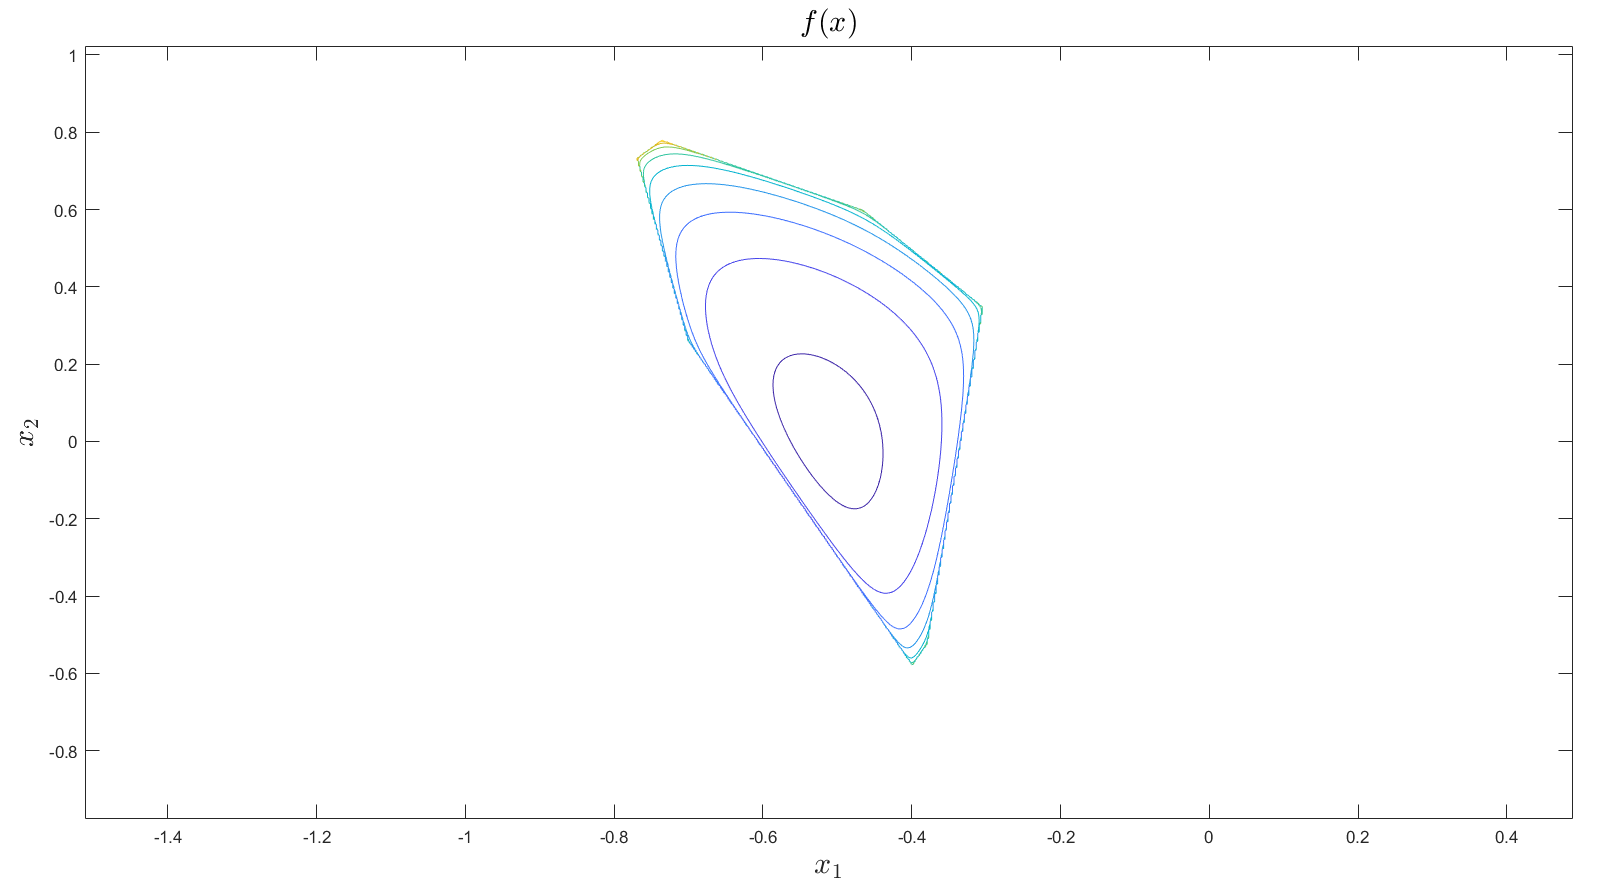
\includegraphics[width=\textwidth]{C_b_2.png}
				\caption{Level Sets of $f$}
			\end{subfigure}
		\end{figure}
		Since for every point that is not in the domain of $f$ we give it an arbitrarily large value we see spike at the edges of the plot.\\
		Also since the domain of $f$ is the intersection of a finite number of inequalities (in the case only one), domain of $f$ is a polyhedron as seen by the level sets.
		
		\item[c]
		We assume that ${\bf x}={\bf 0}$ is a feasible point therefore ${\bf b}>{\bf 0}$.\\
		We apply the gradient algorithm using backtracking line search while concurrently checking if we remain in the domain of f.
		
		\item[d]
		In order to apply the newton algorithm we calculate the hessian matrix. The exit criterion is $\frac{\lambda^2}{2}\leq \epsilon$ where $\lambda^2=\nabla^Tf(\bf x)(\nabla^2f(\bf x))^{-1}\nabla f(\bf x)$ and we set the $dx_k=-(\nabla^2f(\bf x))^{-1}\nabla f(\bf x)$. After we use the backtracking search algorithm while concurrently checking if we remain in the domain of f to find the minima.
		\newpage
		\item[e]
		\begin{figure}
			\centering
			\begin{subfigure}[b]{0.45\textwidth}
				\centering
				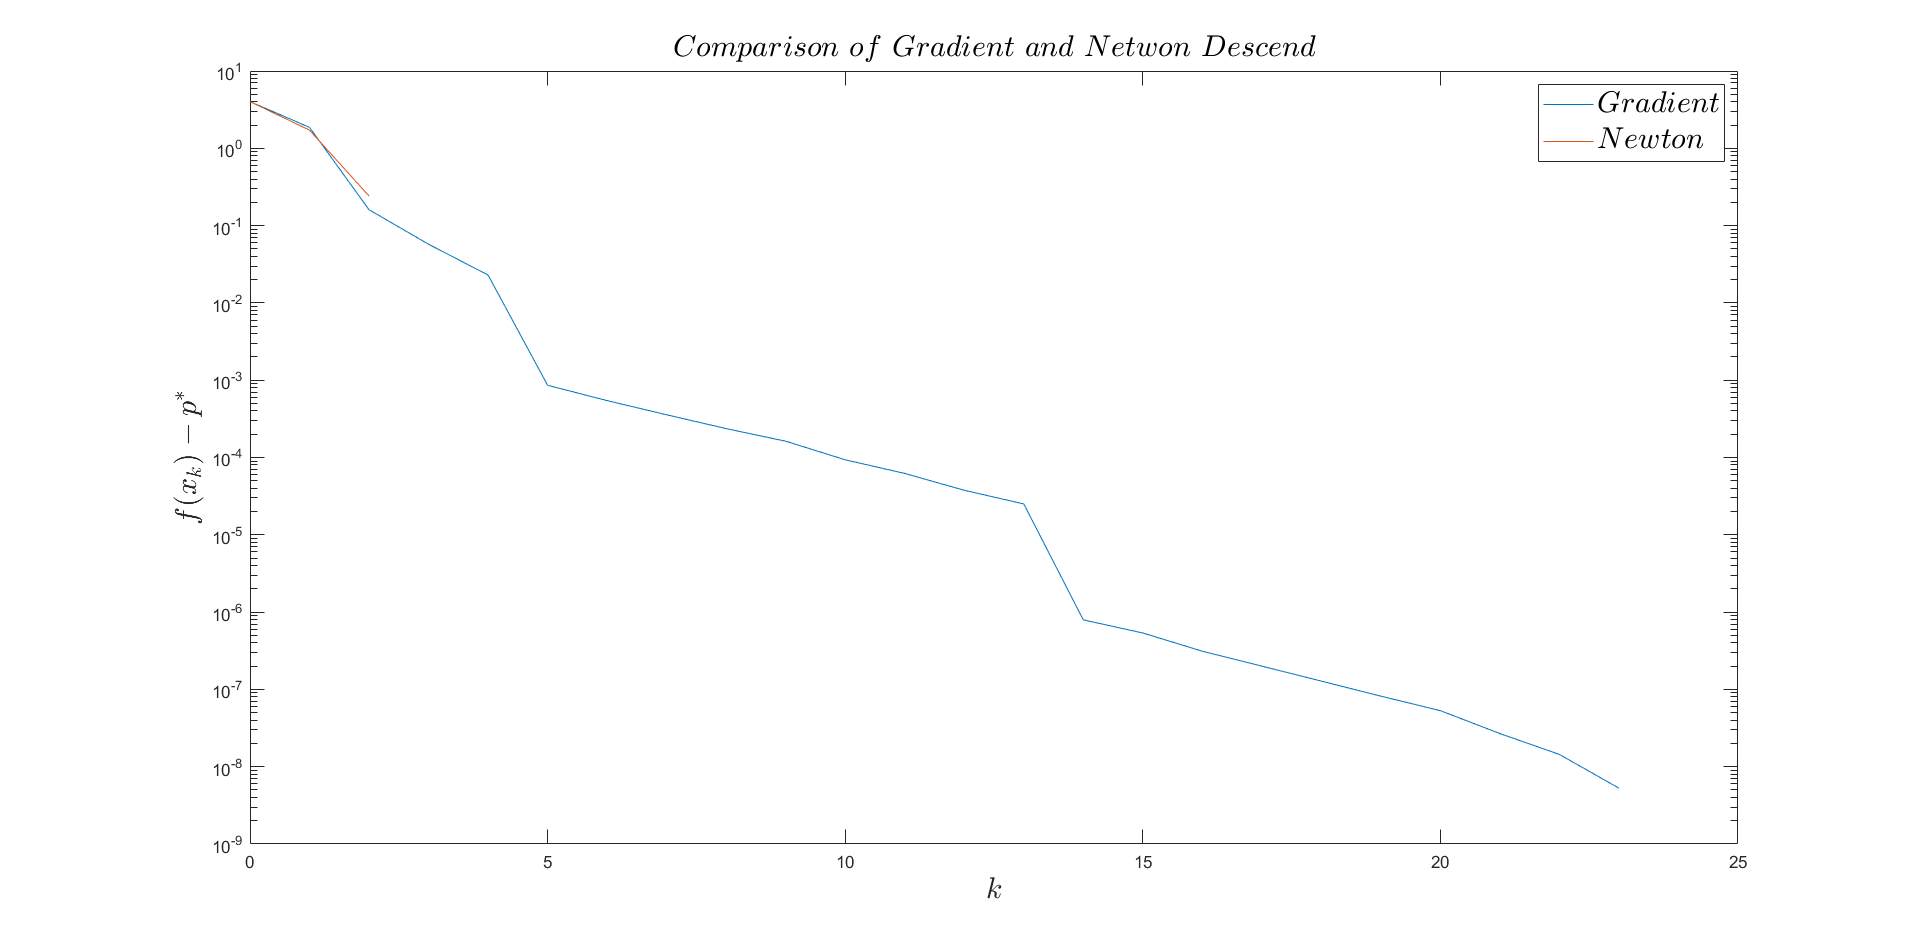
\includegraphics[width=\textwidth]{C_e_1.png}
				\caption{$(n,m)=(2,20)$}
			\end{subfigure}
			\hfill
			\begin{subfigure}[b]{0.45\textwidth}
				\centering
				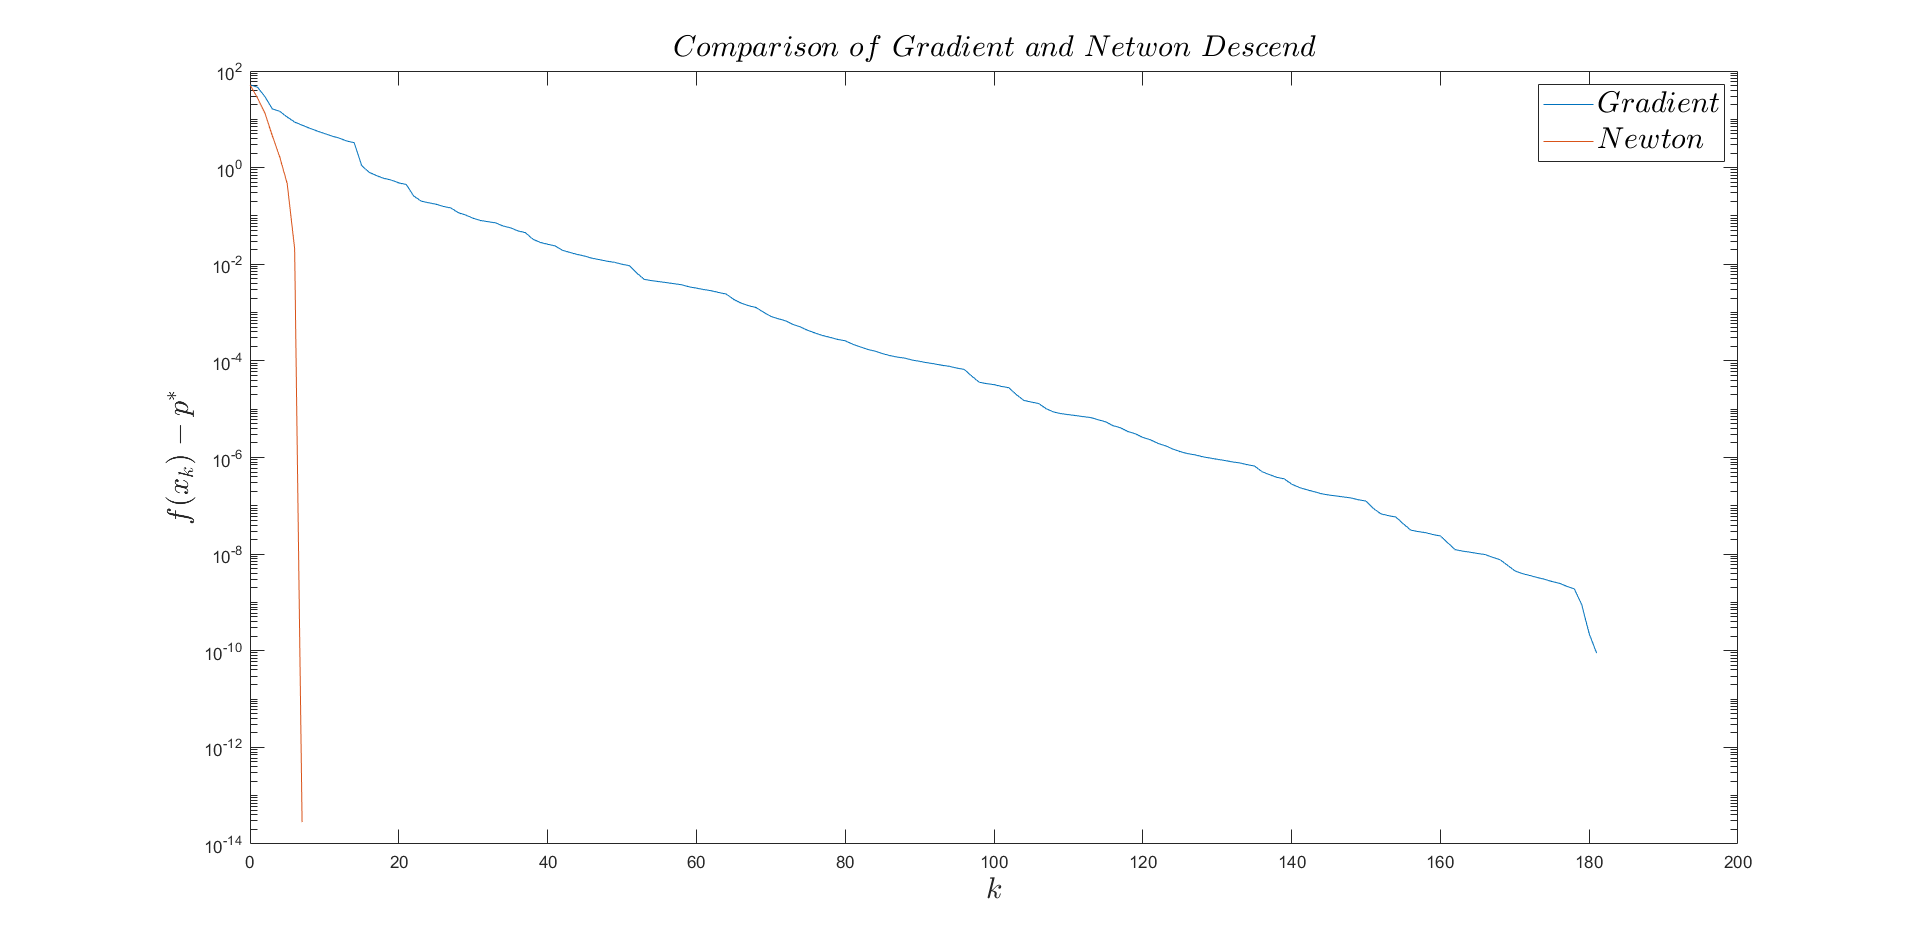
\includegraphics[width=\textwidth]{C_e_2.png}
				\caption{$(n,m)=(50,200)$}
			\end{subfigure}
			\hfill
			\begin{subfigure}[b]{0.45\textwidth}
				\centering
				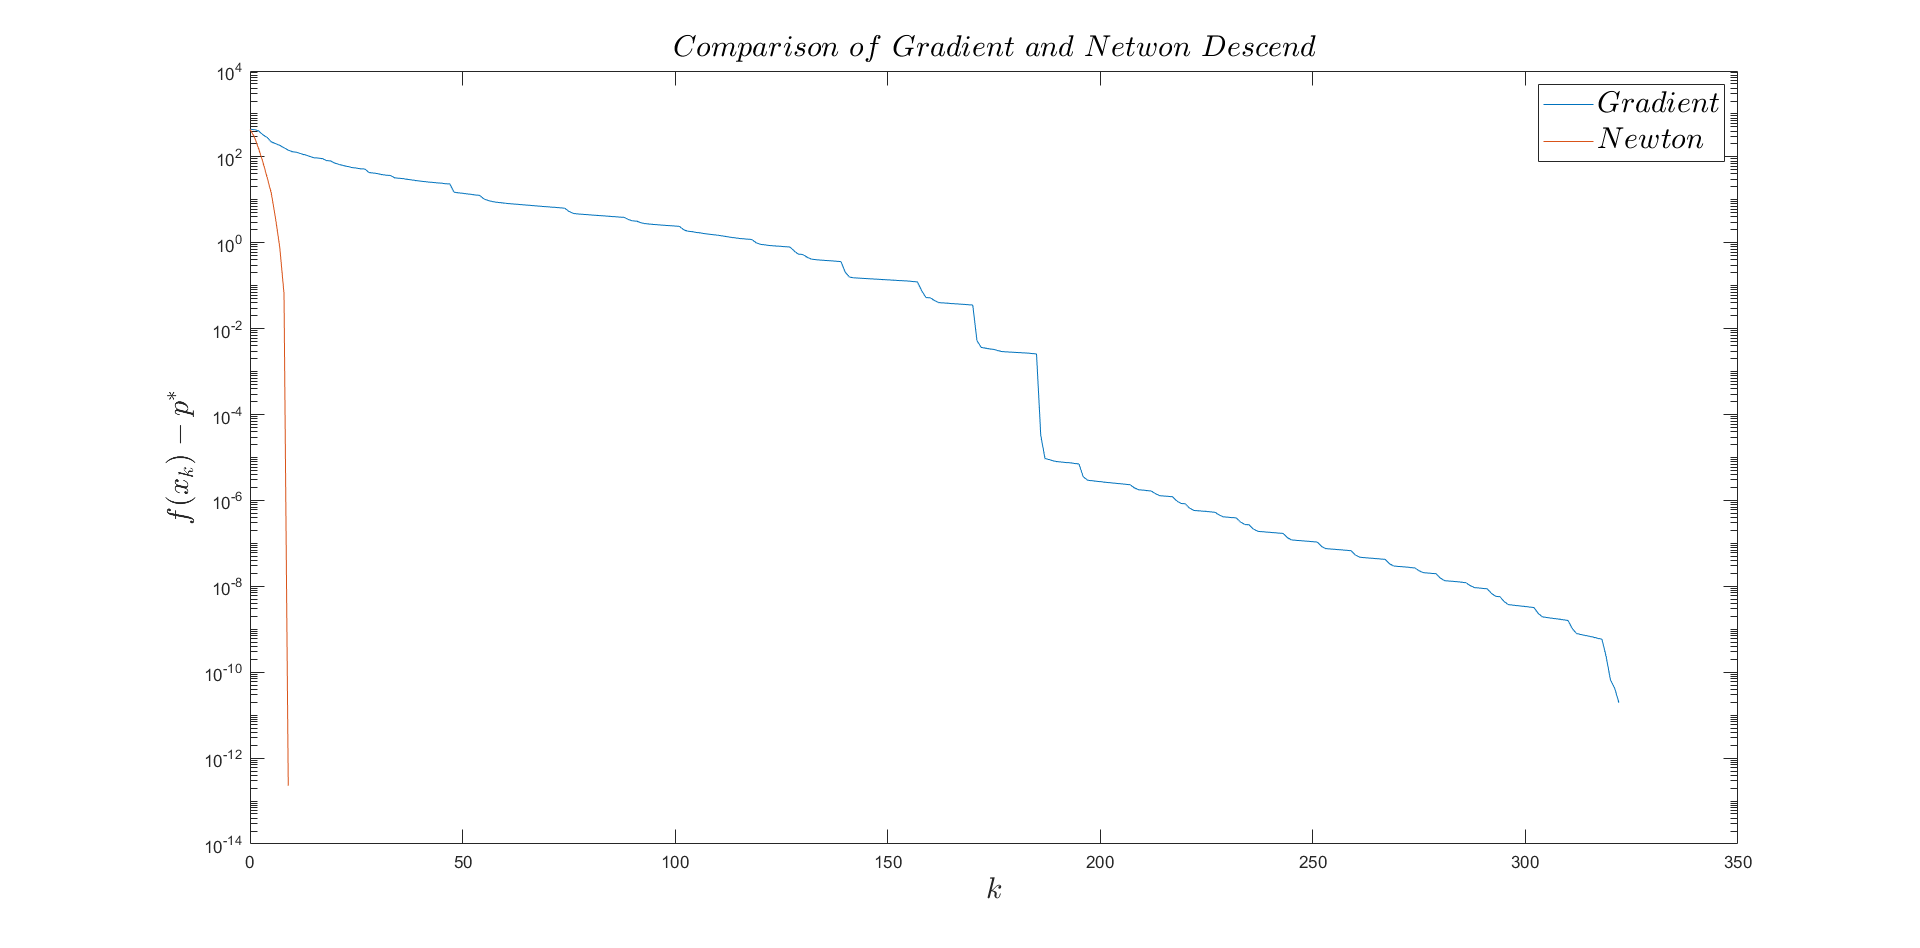
\includegraphics[width=\textwidth]{C_e_3.png}
				\caption{$(n,m)=(300,800)$}
			\end{subfigure}
		\end{figure}
		We can see that the newton descend is always faster than the gradient descend. Although the newton algorithm requires significantly more memory because of the need to calculate the hessian.\\
		It is worth noting ,the reason that an algorithm might seem to end prematurely, by looking the semilogy plots, is that since at their last iteration the algorithms find the optimal value within the error $\epsilon$ and thus the value $f({\bf x}^*)-p^*=0$ and the semilogy function cannot draw that. In reality the algorithms have indeed found the optimal value.
		
		\newpage
		\item[{\bf Code}]
		The matlab code used for the realization of the above experiments.
		{\bf Exercise2.m}: This script contains the code for section B except subsection B.vii
		\lstinputlisting{Exercise2.m}
		
		{\bf Exercise2\_Bvii.m}: This script contains the code for section B.vii.
		\lstinputlisting{Exercise2_Bvii.m}
		
		{\bf Exercise2\_C.m}: This script contains the code for section C.
		\lstinputlisting{Exercise2_C.m}
	\end{enumerate}
	\end{enumerate}
\end{document}
